\documentclass[acmtog]{acmart}
\usepackage{graphicx}
\usepackage{subfigure}
\usepackage{natbib}
\usepackage{listings}
\usepackage{bm}
\usepackage{amsmath}

\definecolor{blve}{rgb}{0.3372549 , 0.61176471, 0.83921569}
\definecolor{gr33n}{rgb}{0.29019608, 0.7372549, 0.64705882}
\makeatletter
\lst@InstallKeywords k{class}{classstyle}\slshape{classstyle}{}ld
%\makeatother
\lstset{language=C++,
    breaklines=true,
%    basicstyle=\ttfamily,
    keywordstyle=\color{blve}\ttfamily,
    stringstyle=\color{red}\ttfamily,
    commentstyle=\color{magenta}\ttfamily,
    morecomment=[l][\color{magenta}]{\#},
    classstyle = \bfseries\color{gr33n},
    tabsize=1,
    morekeywords={Vec3f, Interaction},
}
%\lstset{basicstyle=\ttfamily}


% Title portion
\title{Multi-Resolution Isosurface Rendering}

\author{Name:\quad Bingnan Li \quad Suting Chen \\ student number:\ 2020533092\ 2020533185
\\email:\quad libn@shanghaitech.edu.cn\quad chenst@shanghaitech.edu.cn}

% Document starts
\begin{document}
    \maketitle

    \vspace*{2 ex}


    \section{Related Paper Overview}\label{sec:related-paper-overview}
    In the related paper, they utilized GPU-based structured adaptive mesh refinement to save computational time and storage for rendering scientific simulation data efficiently.
    The key contribution of the article is to reorganize multi-level AMR data so that data, especially its boundaries can be accessed efficiently enough.
    They also worked on adaptive sampling on the volume for color and opacity.
    \begin{enumerate}
        \item ExaBricks
        \par In their actual implementation, they use BVH with hardware acceleration for their data structure, named `ExaBricks`.
        \par By contrast, we harnessed OpenVDB, a well-design OC-tree for keeping data to visualize, enables fast traversal through a specific layer. To search for the exact layers of voxels, we implemented KD-tree for acceleration.
        \item Sampling
        \par Each metadata is leveraged to adapt the sampling rate when traversing for matching the frequency of the data it contains.
        \item Rendering
        \par First trace each ray against the BVH, then transform it into the volume space, and trace it against the iso-surface BVH to check for a closer surface hit point.
        Then, the ray is shortened to the nearest interaction point. Ambient occlusion is also supported in addition to local shading.
    \end{enumerate}


    \section{Introduction}\label{sec:introduction}
    \begin{itemize}
        \item data preprocessing
        \item k-d tree
        \item transfer function
        \item Interpolation
        \item volume rendering
        \item object rendering and object filtering
    \end{itemize}


    \section{Implementation Details}\label{sec:implementation-details}

    \subsection{data preprocessing}\label{subsec:data-preprocessing}
    In this project, we dealt with \emph{.vdb} files and try to visualize four different multi-resolution grids.
    In order to accomplish that, we utilized \emph{openvdb} library to read the \emph{.vdb} files and extract the grids.F
    Given that the vdb grids are actually velocity field around a sphere which is a vector field, we need to perform scalarization:
    \begin{enumerate}
        \item Turn the velocity field into a scalar field by using the magnitude of the velocity field.
        \item Calculate the q-criteria of the velocity field.
        \par Q-criteria is a scalar field that is used to determine the quality of the flow.
        It is defined as:
        \begin{equation}
            Q = -\frac{1}{2}\left( \left( \frac{\partial u}{\partial x} \right)^2 + \left( \frac{\partial v}{\partial y} \right)^2 + \left( \frac{\partial w}{\partial z} \right)^2 \right) - \frac{\partial u}{\partial y}\frac{\partial v}{\partial x} - \frac{\partial u}{\partial z}\frac{\partial w}{\partial x} - \frac{\partial v}{\partial z}\frac{\partial w}{\partial y}\label{eq:equation}
        \end{equation}
        where $u$, $v$, $w$ are the velocity components in the $x$, $y$, $z$ directions respectively.
        \par As for calculating the gradient, we use the \emph{Central Finite Difference Approximations}, which defines as follows:
        \begin{align*}
            f'(x)=\frac{f(x+h)-f(x-h)}{2h}
        \end{align*}
        with ths approximation, we can efficiently calculate the q-criteria from a discrete velocity field.
        \par Moreover, q-criteria field has a property that the gradient always points to the interior of the flow, which is useful when designing the transfer function.
    \end{enumerate}

    The code of generating q-criteria grids are as follows:
    \begin{lstlisting}[label={lst:lstlisting7}]
void Scene::genQGrids() {
    for (const auto &grid: vectorGrids) {
        float dx = (float) (grid->transform().voxelSize()[0]);
        auto qGrid = floatGrid::create();
        qGrid->setTransform(grid->transform().copy());
        qGrid->topologyUnion(*grid);
        auto accessor = qGrid->getAccessor();
        auto vec_accessor = grid->getAccessor();
        for (auto iter = grid->cbeginValueOn(); iter; ++iter) {
            float qValue = 0.0f;
            openvdb::Coord ijk = iter.getCoord();
            openvdb::Coord low_x = ijk + openvdb::Coord{-1, 0, 0}, low_y = ijk + openvdb::Coord{0, -1, 0},
                    low_z = ijk + openvdb::Coord{0, 0, -1};
            openvdb::Coord high_x = ijk + openvdb::Coord{1, 0, 0}, high_y = ijk + openvdb::Coord{0, 1, 0},
                    high_z = ijk + openvdb::Coord{0, 0, 1};
            Vec3f grad_x = (vec_accessor.getValue(high_x) - vec_accessor.getValue(low_x)) / (2 * dx);
            Vec3f grad_y = (vec_accessor.getValue(high_y) - vec_accessor.getValue(low_y)) / (2 * dx);
            Vec3f grad_z = (vec_accessor.getValue(high_z) - vec_accessor.getValue(low_z)) / (2 * dx);

            qValue = -0.5f * (grad_x[0] * grad_x[0] + grad_y[1] * grad_y[1] + grad_z[2] * grad_z[2]) -
                     grad_y[0] * grad_x[1] - grad_z[0] * grad_x[2] - grad_z[1] * grad_y[2];
            accessor.setValue(iter.getCoord(), qValue);
        }
        QGrids.push_back(qGrid);
    }
}
    \end{lstlisting}

    \subsection{k-d tree}\label{subsec:k-d-tree}
    k-d tree is implemented to display various layers of resolutions, each layer divides the space into parts (mostly 7 in our case).
    The tree is utilized to search for the resolution layers supporting a voxel.
    \begin{enumerate}
        \item Constructing the tree from scratch is simple: each resolution is read from a separate file, from which a bounding box and their intersection can be calculated. In our case, lower resolution always have a bounding box that contains higher resolution area. Hence, each level of KD-tree includes the next level of KD-tree with its surroundings.
        \item Traversing the tree to search for dependency from the top:
        \par If current level is already leaf, return dependency for current level.
        \par Else we traverse the layer, and search for the voxel according to the bounding boxes.
        \par Recursively search through every layer, until a leaf node is found or no leaf node is found to be satisfying.
    \end{enumerate}
    There are some limitations on our design. Due to the low complexity of the model, we assert layers' have a bounding box that contains each other.
    In real engineering cases, the distribution can be arbitrary. Hence its not efficiency enough to count the whole bounding box as support region.

    \subsection{transfer function}\label{subsec:transfer-function}
    In this project, we use different scalar field to map scalar to color and opacity.
    For opacity, we use q-criteria as the input of transfer function.
    Next, we will show the detail of opacity transfer function:
    Assume that we want to visualize the q-criteria with iso-value $i$, then we set opacity as follows:
    \begin{align*}
        opacity = \left\{
        \begin{aligned}
            1&\quad if\ q \geq i\\
            0&\quad elsewhere
        \end{aligned}
        \right.
    \end{align*}
    The reason why we can simply set opacity above has been mentioned in~\ref{subsec:data-preprocessing}, since the gradient of q-criteria field always points to the interior of the iso-surface, we know that the iso-value of interior side is always larger than the exterior side.
    Based on that, if we use \emph{front-to-back} algorithm to perform volume rendering and apply \emph{early termination} like
    \begin{lstlisting}[label={lst:lstlisting}]
        if (src_opacity > 1 - 1e-2) break;
    \end{lstlisting}
    we can guarantee the correctness of the rendering result and in the meanwhile, achieve efficiency.

    For color, we use module of velocity field as the input of transfer function.
    We perform a linear interpolation between four colors with the following procedure:

    We first divided the range of the module of velocity field into four parts, and then we set the color of each part as follows:

    Assume we are in part $[m_0, m_1]$ and get module $m$, and the corresponding color of $m_0,m_1$ are $c_0, c_1$ resp.~ then the the corresponding color of $m$ is
    \[c=\frac{m_1-m}{m_1-m_0}\times c_0 + \frac{m-m_0}{m_1-m_0}\times c_1\]
    ]
    The corresponding codes are as follows:

    Opacity:
    \begin{lstlisting}[label={lst:lstlisting4}]
float Scene::sampleOpacity(float value) {
    if (value > isoValue) {
        return 1;
    } else {
        return 0;
    }
}
    \end{lstlisting}

    Color:

    \begin{lstlisting}[label={lst:lstlisting5}]
Vec3f Scene::sampleEmission(float value, float opacity) const {
    float a_coef = 0, b_coef = 0, c_coef = 0, d_coef = 0;
    float mid_value_1 = (max_value + min_value) / 3;
    float mid_value_2 = 2 * mid_value_1;
    Vec3f A{0, 0.9, 0.2}, B{0.8, 0.8, 0}, C{1, 0, 0}, D{0.4, 0.6, 0};
    if (value < mid_value_1) {
        float range = mid_value_1 - min_value;
        a_coef = 1 - (value - min_value) / range;
        b_coef = 1 - (mid_value_1 - value) / range;
    } else if (value >= mid_value_1 && value < mid_value_2){
        float range = mid_value_2 - mid_value_1;
        b_coef = 1 - (value - mid_value_1) / range;
        c_coef = 1 - (mid_value_2 - value) / range;
    } else {
        float range = max_value - mid_value_2;
        c_coef = 1 - (value - mid_value_2) / range;
        d_coef = 1 - (max_value - value) / range;
    }
    auto color = a_coef * A + b_coef * B + c_coef * C + d_coef * D;
    if (opacity < 1e-3) {
        return {0, 0, 0};
    } else {
        return color ;
    }
}
    \end{lstlisting}

    \subsection{Interpolation}\label{subsec:interpolation}
    Given that vdb files are all discrete voxels and ray marching algorithm ask as to access data in any world coordinate.
    In order to solve this problem, we need to perform interpolation within multi-resolution grids.

    For simply case, when we only have single resolution, we need to calculate a hat-shaped basis function:
    \begin{equation}
        \hat{H}_C(p) = \hat{h}\left( \frac{|C_{px}-p_x|}{C_w} \right)\hat{h}\left( \frac{|C_{py}-p_y|}{C_w} \right)\hat{h}\left( \frac{|C_{pz}-p_z|}{C_w} \right)\label{eq:equation2}
    \end{equation}
    where $\hat{h}(x) = \max(1-x,0) $, $C_w$ is the width of cell $C$ and $C_{px}, C_{py}, C_{pz}$ are the coordinate along three axis.
    Then, for reconstructing a sample at position $p$, we need to involve all cell $C_i$ with value $C_{v_i}$ such that $\hat{H}_{C_i}(p) \neq 0$ and compute the weighted sum:
    \begin{equation}
        B(p)=\frac{\sum_{C_i} \hat{H}_{C_i}(p)C_{v_i}}{\sum_{C_i}\hat{H}_{C_i}(p)}\label{eq:equation3}
    \end{equation}

    However, for a more complicated case, if we have multi-resolution grids, we need to use k-d tree to first determine which resolutions do we need to preform interpolation.
    Then we calculate the multi-interpolation with the procedure shown above.

    Then corresponding codes are as follows:
    \begin{lstlisting}[label={lst:lstlisting6}]
template<typename T, typename GridType>
int Scene::interpolation(const Vec3f &pos, T &res, const std::vector<GridType> &Grids) const {
    std::vector<std::vector<Vec3i>> Corners;
    for (const auto &grid: Grids) {
        Vec3d local_pos = (grid->transform().worldToIndex(pos));
        Vec3i lower = {Vec3i(floor(local_pos.x()), floor(local_pos.y()), floor(local_pos.z()))};
        Vec3i upper = {Vec3i(ceil(local_pos.x()), ceil(local_pos.y()), ceil(local_pos.z()))};
        Corners.push_back(
        {{lower.x(), lower.y(), lower.z()},
        {lower.x(), lower.y(), upper.z()},
        {lower.x(), upper.y(), lower.z()},
        {lower.x(), upper.y(), upper.z()},
        {upper.x(), lower.y(), lower.z()},
        {upper.x(), lower.y(), upper.z()},
        {upper.x(), upper.y(), lower.z()},
        {upper.x(), upper.y(), upper.z()}});
    }

    res = T(0);

    // Traverse KD-tree
    int layers = searchTree(pos);
    if (layers == -1) return -1;

    T numerator(0);

    float denominator = 0;
    for (int r = 0; r < 8; ++r) {
        for (int i = layers; i >= 0; --i) {
            openvdb::Coord coord{Corners[i][r]};
            float dx = float(Grids[i]->transform().voxelSize()[0]);
            if (Grids[i]->tree().isValueOn(coord)) {
                Vec3f corner = Grids[i]->transform().indexToWorld(Corners[i][r]);
                float weight = 1;
                for (int j = 0; j < 3; j++) {
                    weight *= float(fmax((1 - fabs(corner[j] - pos[j]) / dx), 0.0));
                }
                numerator += weight * Grids[i]->tree().getValue(coord);
                denominator += weight;
                break;
            }
        }
    }
    if (denominator != 0) res = numerator / denominator;
    return layers;
}
    \end{lstlisting}

    \subsection{volume rendering}\label{subsec:volume-rendering}
    For the volume rendering part, we use \emph{front-to-back} algorithm to rendering the turbulence.
    The procedure of \emph{front-to-back} algorithm is as follows:
    \begin{itemize}
        \item Initialize destination opacity and destination color to 0.
        \item Marching \emph{step\_size} length along the ray and get the source opacity and color.
        \item Accumulate opacity and color with the following formulas:
        \begin{align*}
            C_{dst} &= C_{dst} + (1-\alpha_{dst}) \times C_{src}\\
            \alpha_{dst} &= \alpha_{dst} + (1-\alpha_{dst})\times \alpha_{src}
        \end{align*}
        where $C_{dst}, C_{src}$ are the color of destination and source resp.~ and $\alpha_{dst}, \alpha_{src}$ are the opacity of destination and source resp.
        \item Once we march beyond limit or the source opacity $> 0.99$ , we terminate.
    \end{itemize}
    We attached the code:
    \begin{lstlisting}[label={lst:lstlisting2}]
float step_size = scene->grids[0].dx / 16;
Vec3f src_color;
float src_opacity;
auto src_t = (float) fmax(t0 - step_size, ray.t0());
Vec3f src_pos, dst_color = Vec3f{0, 0, 0};
float dst_opacity = 0;
float dx;
while (src_t < t1) {
    src_t += step_size;
    src_pos = ray(src_t);
    std::tie(src_color, src_opacity, dx) = scene->getEmissionOpacity(src_pos);
    step_size = dx / 16;
    src_opacity = (float) (1.0 - std::pow(1 - src_opacity, step_size));
    dst_color += (1 - dst_opacity) * src_color;
    dst_opacity += (1 - dst_opacity) * src_opacity;
    if (src_opacity > 1 - 1e-2) break;
}
return {dst_color, dst_opacity};
    \end{lstlisting}

    \subsection{object rendering and object filtering}\label{subsec:object-rendering-and-object-filtering}
    In this project, we use surface rendering (a.k.a.~ object rendering) to visualize the sphere that the wind passes through.
    This model is a simple phong-lighting model and ray-casting model but with slightly change in oder to match volume rendering:
    Beyond the simple phong-lighting model, we check whether the ray touches the volume part first by checking whether the destination opacity is larger than zero.

    We achieve this part by the following procedure: we first perform an object filtering by apply ray-sphere intersection to find the limit of marching depth.
    In order to achieve a acceptable result, we slightly dilated the radius of the sphere to ensure that all the volumes are covered by the sphere.
    Then for the rendering part, we applied another ray-sphere intersection but with the correct sphere radius in order to render the real size of the sphere.
    After that, we perform volume rendering with the marching depth determined during the first ray-sphere intersection.
    However, even this procedure can vanish most volumes attach to the sphere, there are still tiny pitches that levitate above the sphere.
    In order to solve those pitches, we adjust the size of bounding box so that those pitches are beyond the bounding box.

    For each pixel in the output image, we perform the following code:
    \begin{lstlisting}[label={lst:lstlisting3}]
Vec3f L(0, 0, 0);
float t0, t1, t_max = 1e10;
Vec3f phongColor(0);
Interaction interaction;
if (scene->sphere.aabb.intersect(ray, t0, t1)) {
   if (scene->dilated_sphere.intersect(ray, interaction)) {
       t_max = interaction.dist;
       if (scene->sphere.intersect(ray, interaction)) {
           phongColor = radiance(ray, interaction, Vec3f{4, 1.5, 0});
       }
   }
}
if (scene->grids[0].aabb.intersect(ray, t0, t1)) {
    auto colorOpacity = radiance(ray, t0, std::min(t1, t_max));
    L += colorOpacity.first;
    if (colorOpacity.second < 1 - 1e-3) {
        L += phongColor;
    }
} else {
    L += phongColor;
}
camera->getImage()->setPixel(dx, dy, L);
    \end{lstlisting}


    \section{Results}\label{sec:results}
    This part we will show the rendering results for different models and with different rendering configurations.

    \subsection{multi-resolution big model}\label{subsec:multi-resolution-big-model}
    \begin{figure}[H]
        \centering
        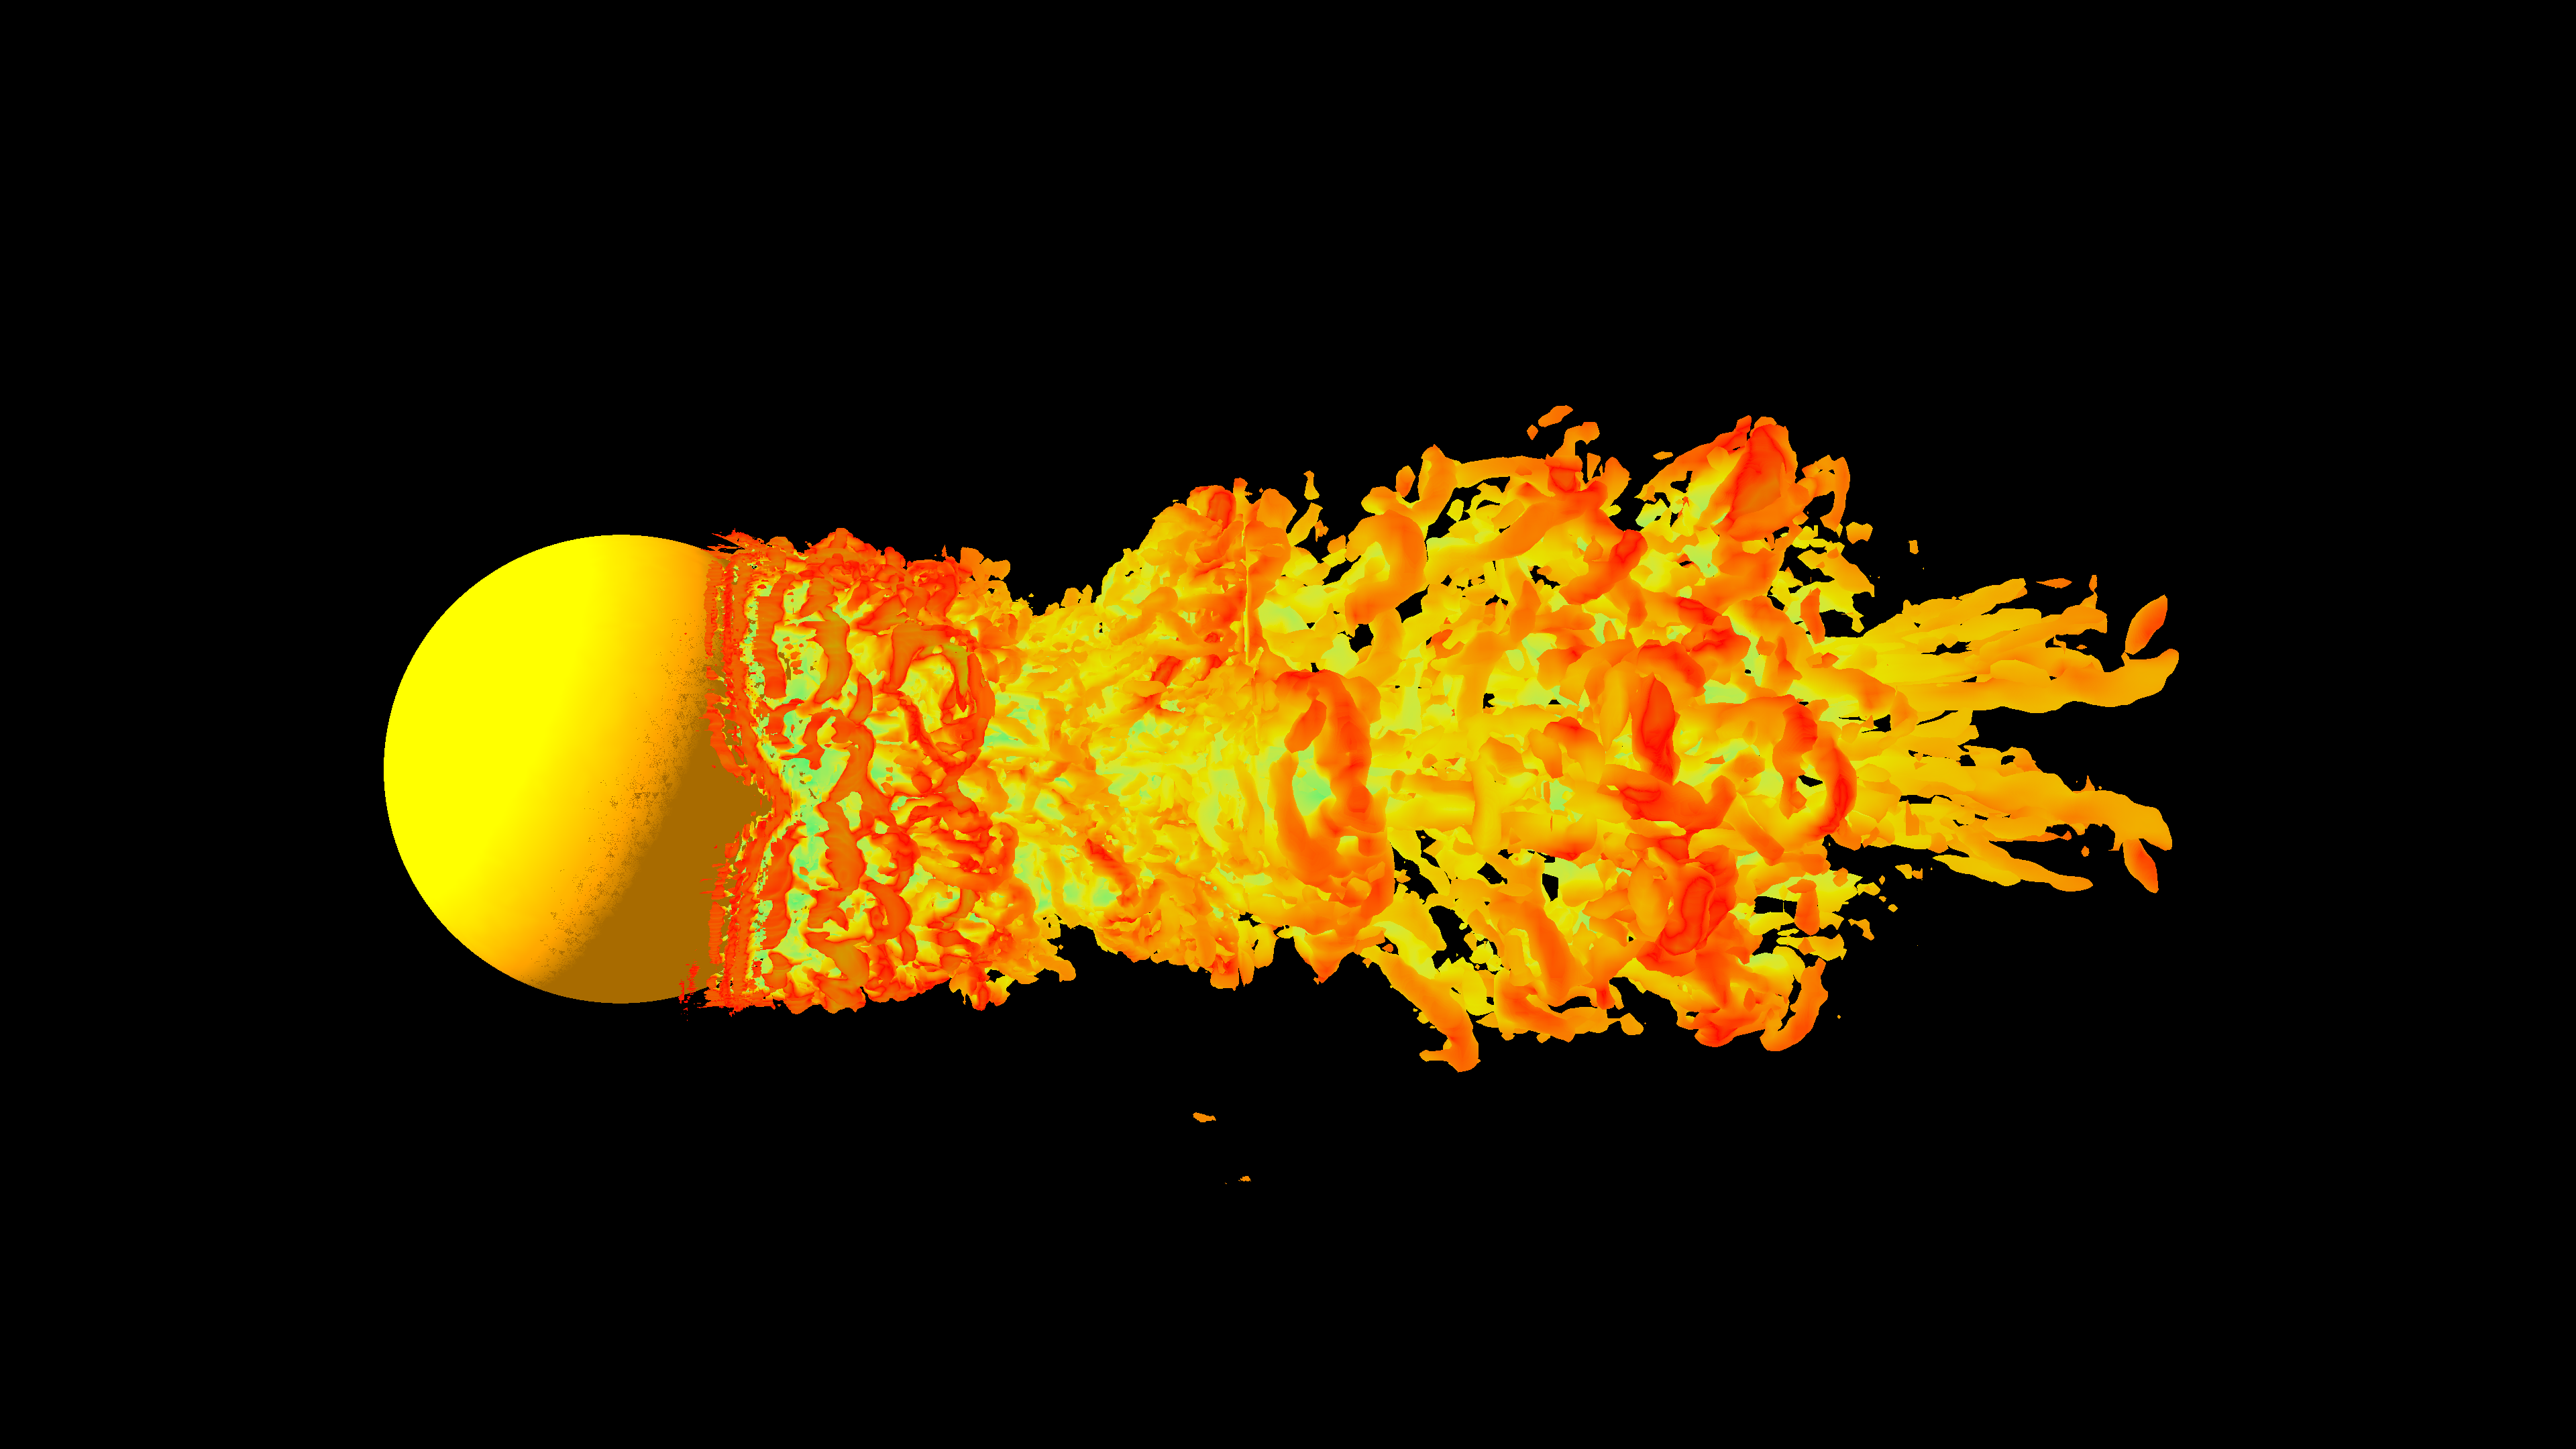
\includegraphics[width=0.45\textwidth]{./image/multi_big_4k_8_filter_0.02}
        \caption{Multi-resolution big field, 4k resolution, $ \frac{dx}{8} $ step size with object filtering (iso-value = 0.02)}\label{fig:figure1}
    \end{figure}

    \begin{figure}[H]
        \centering
        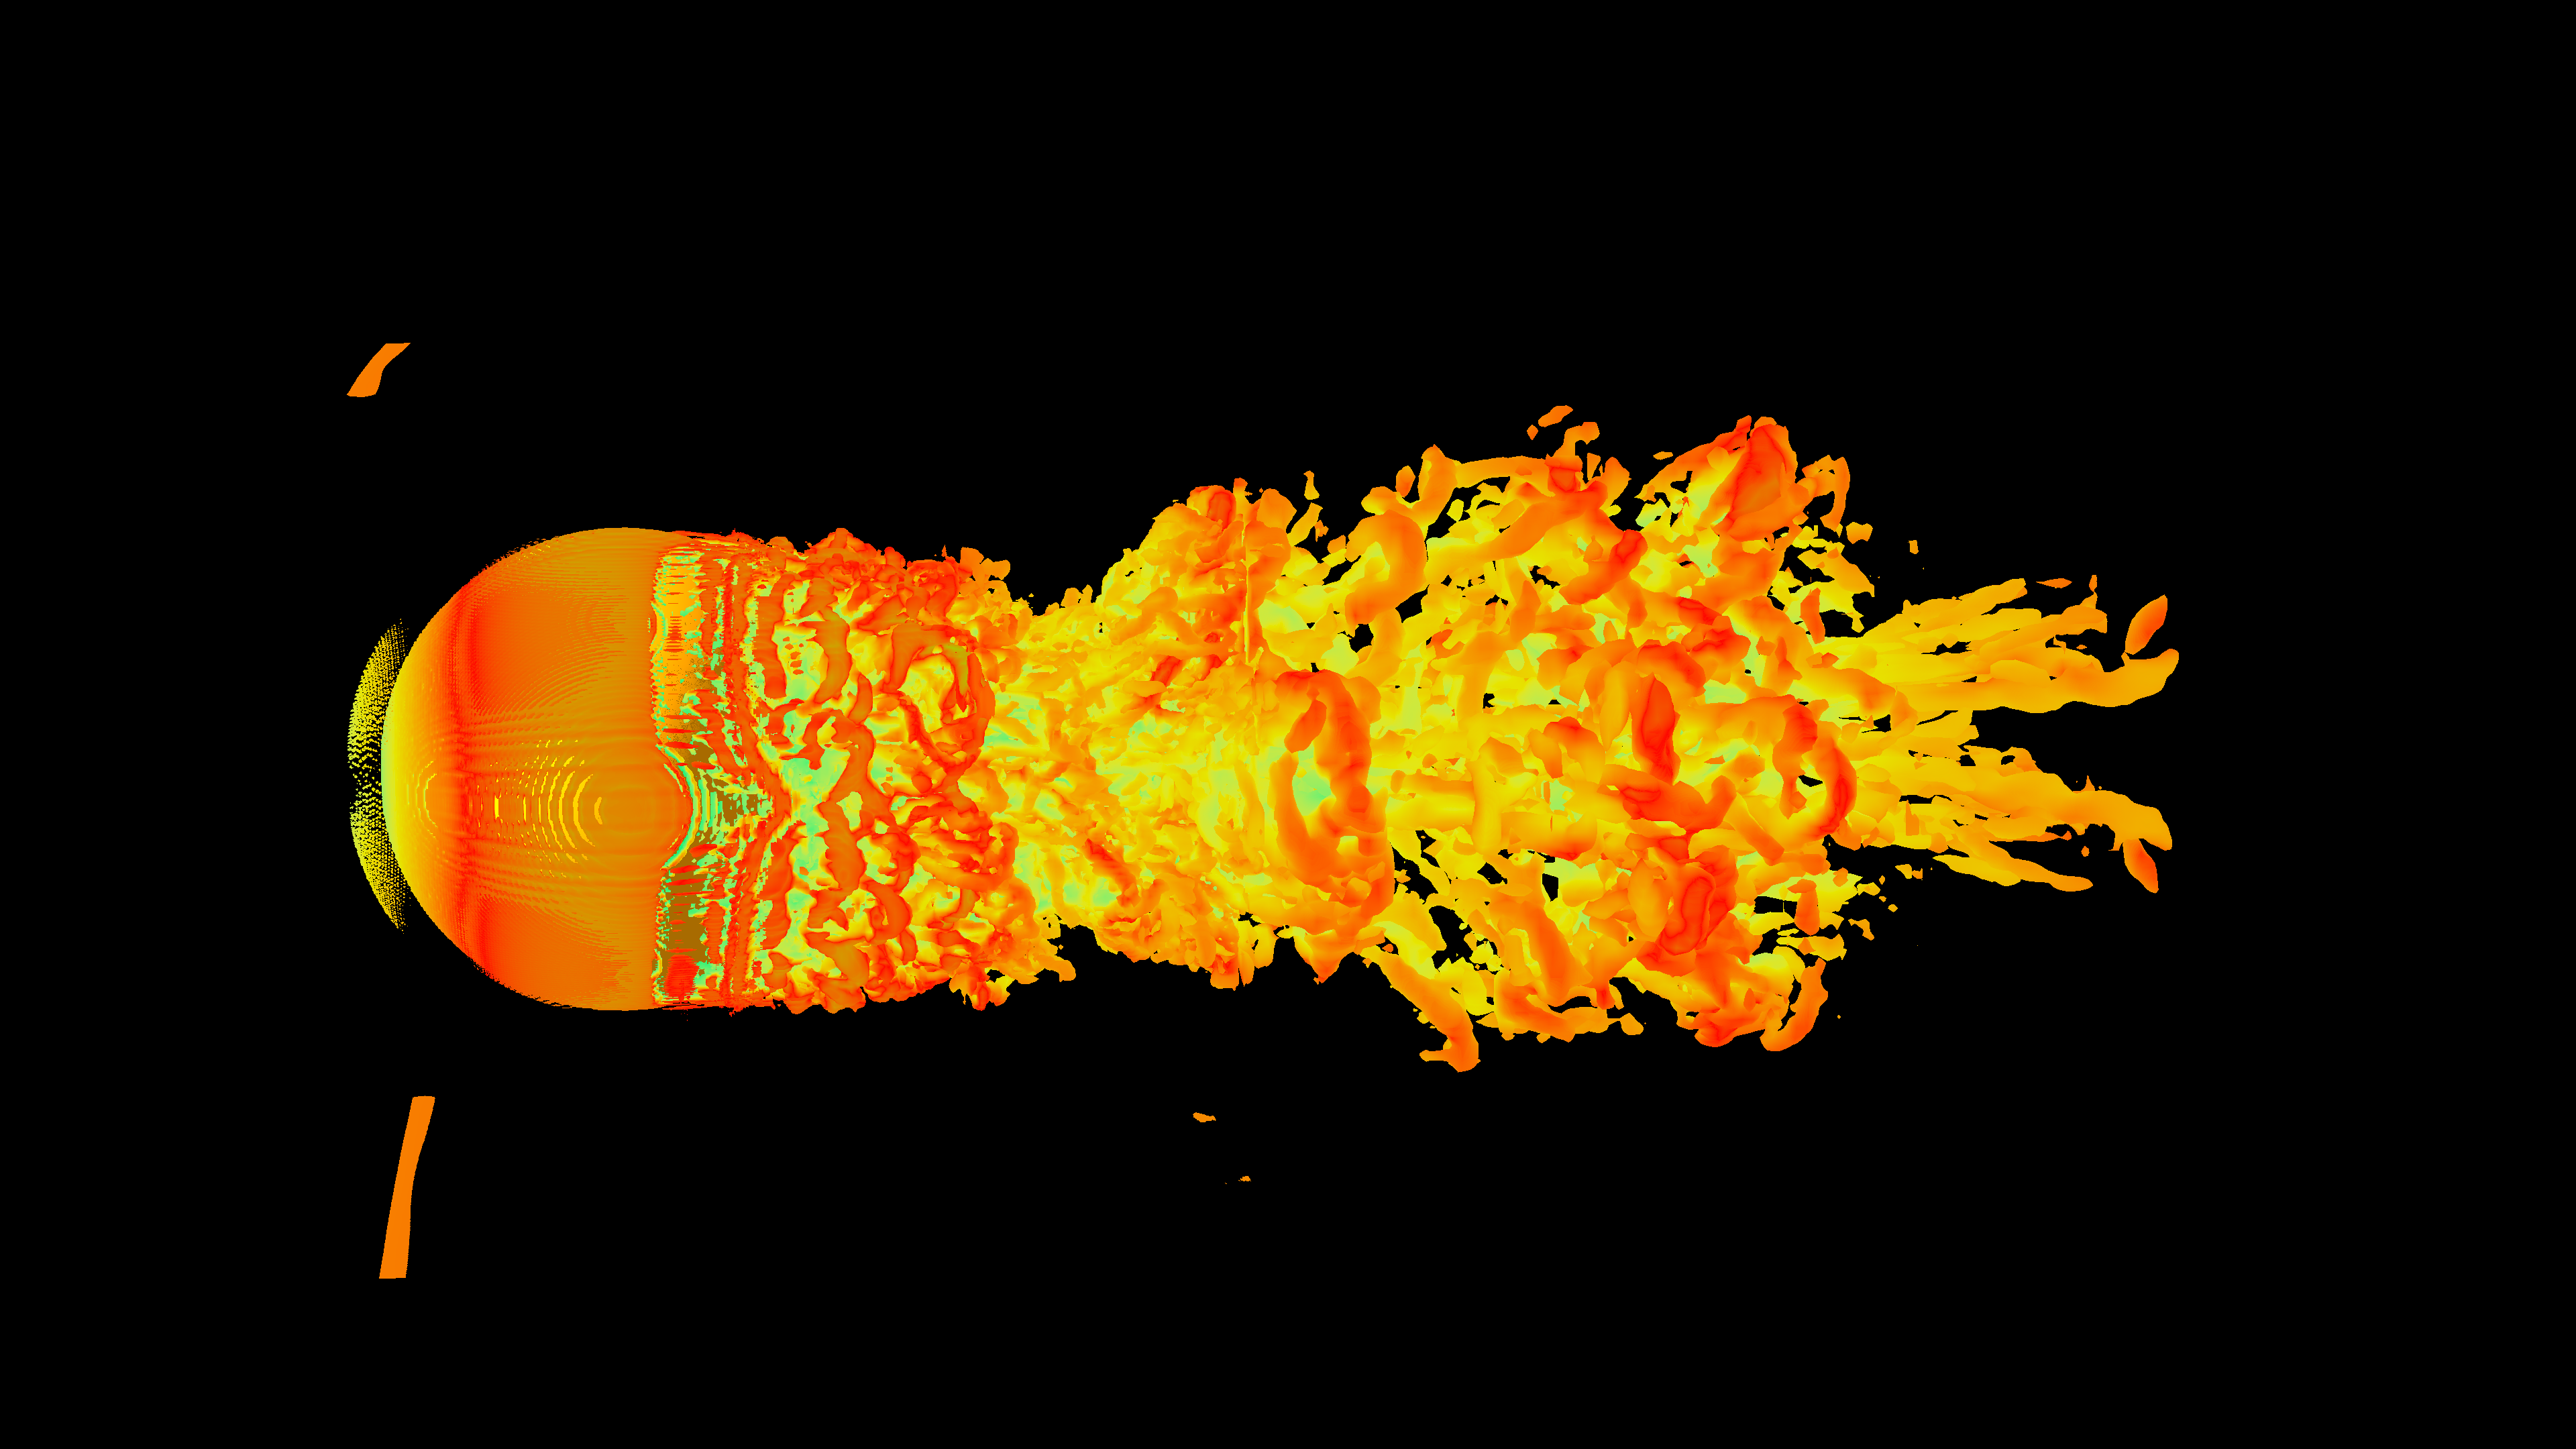
\includegraphics[width=0.45\textwidth]{./image/multi_big_4k_8_no_filter_0.02}
        \caption{Multi-resolution big field, 4k resolution, $ \frac{dx}{8} $ step size without object filtering (iso-value = 0.02)}\label{fig:figure2}
    \end{figure}

    \begin{figure}[H]
        \centering
        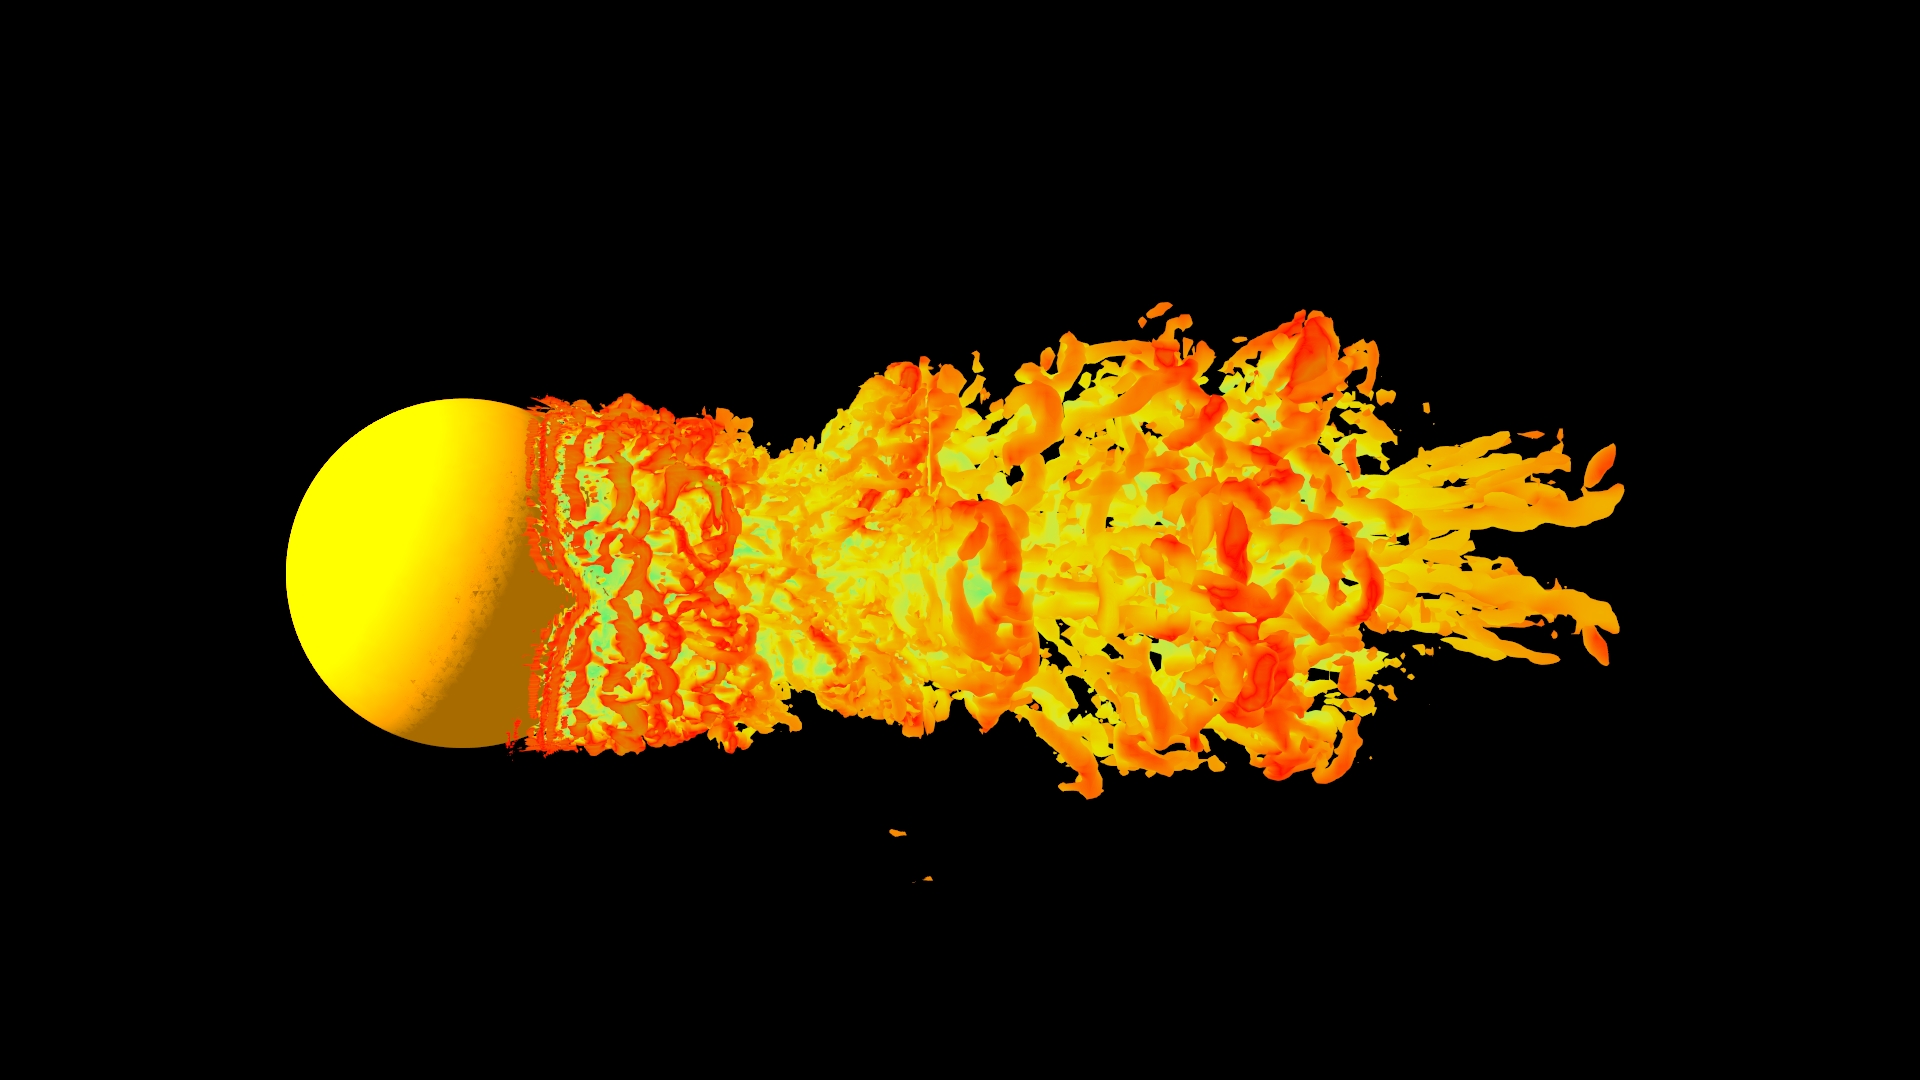
\includegraphics[width=0.45\textwidth]{./image/multi_big_1080p_8_filter_0.02_4XRES}
        \caption{Multi-resolution big field, 1080p resolution, $ \frac{dx}{8} $ step size with object filtering and 4X super resolution anti-aliasing (iso-value = 0.02)}\label{fig:figure3}
    \end{figure}

    \begin{figure}[H]
        \centering
        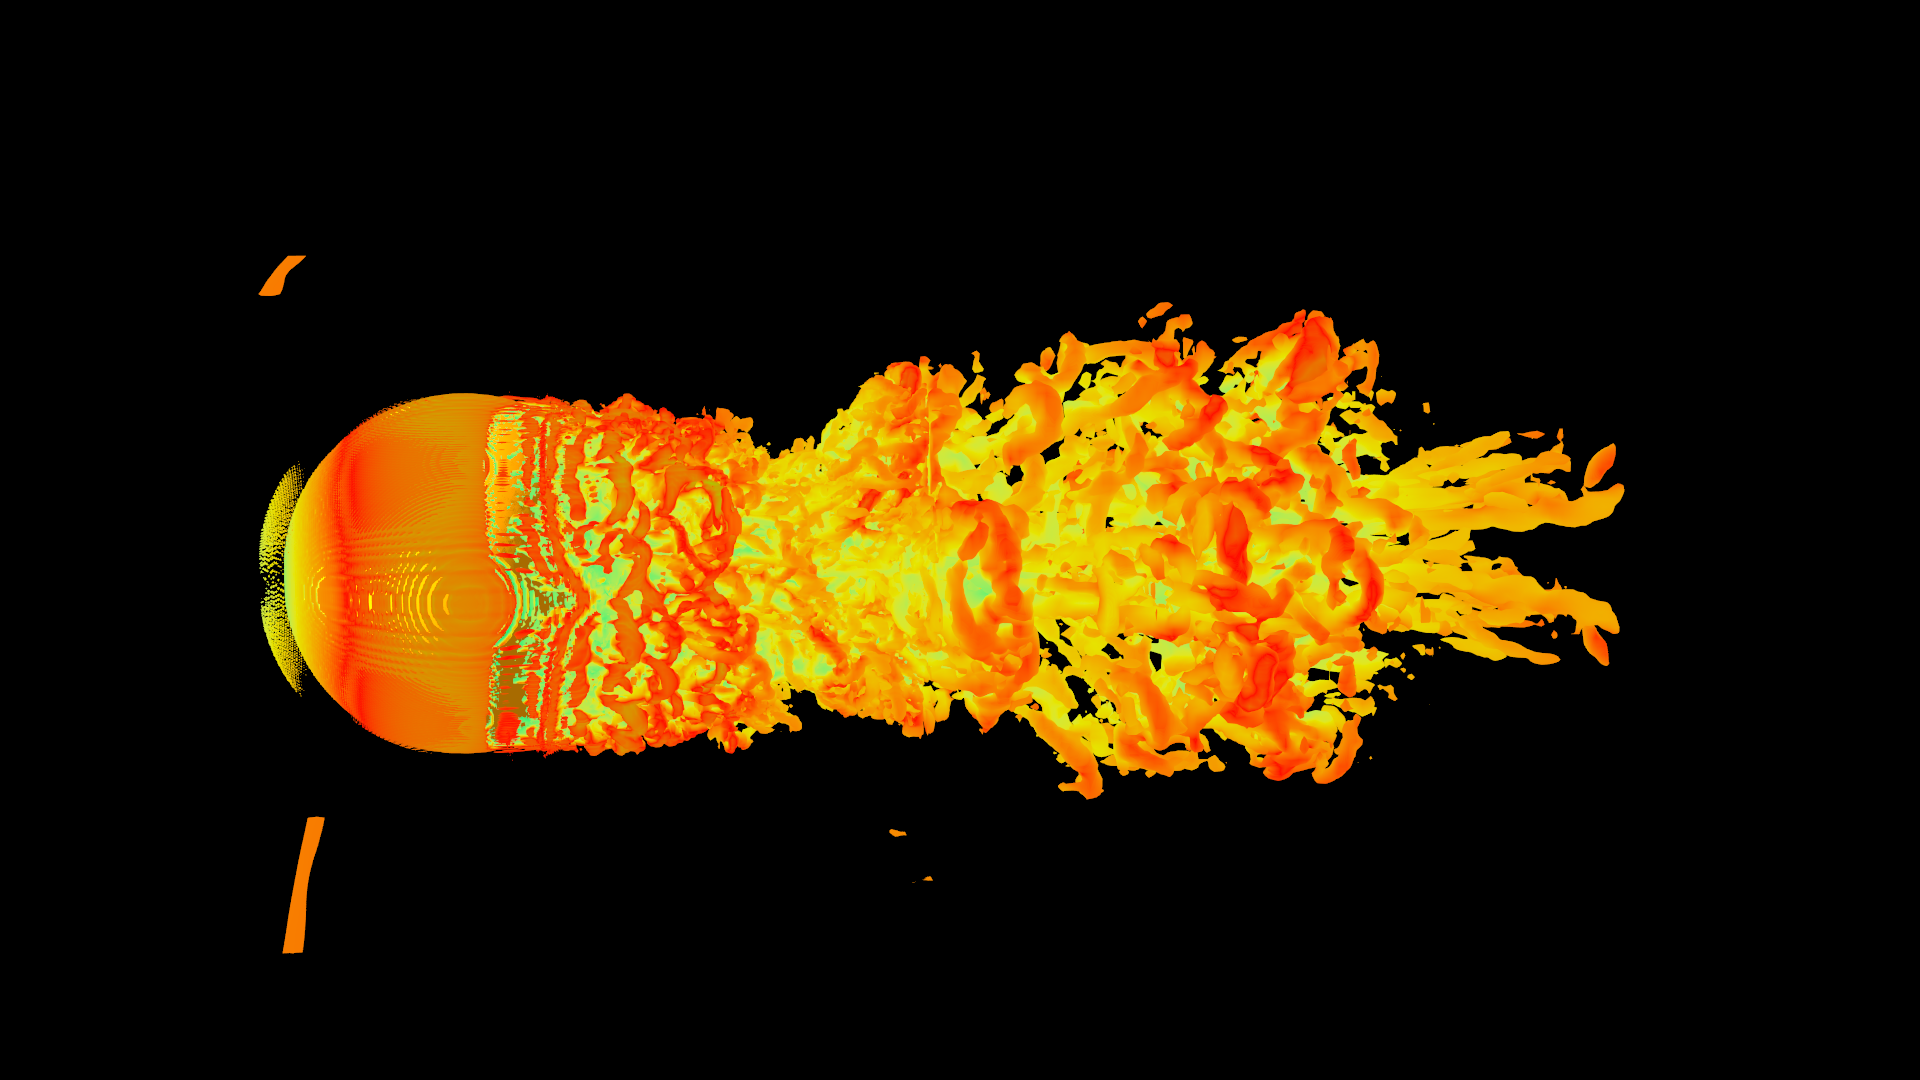
\includegraphics[width=0.45\textwidth]{./image/multi_big_1080p_8_no_filter_0.02_4XRES}
        \caption{Multi-resolution big field, 1080p resolution, $ \frac{dx}{8} $ step size without object filtering and 4X super resolution anti-aliasing  (iso-value = 0.02)}\label{fig:figure4}
    \end{figure}

    \subsection{multi-resolution small model}\label{subsec:multi-resolution-small-model}
    \begin{figure}[H]
        \centering
        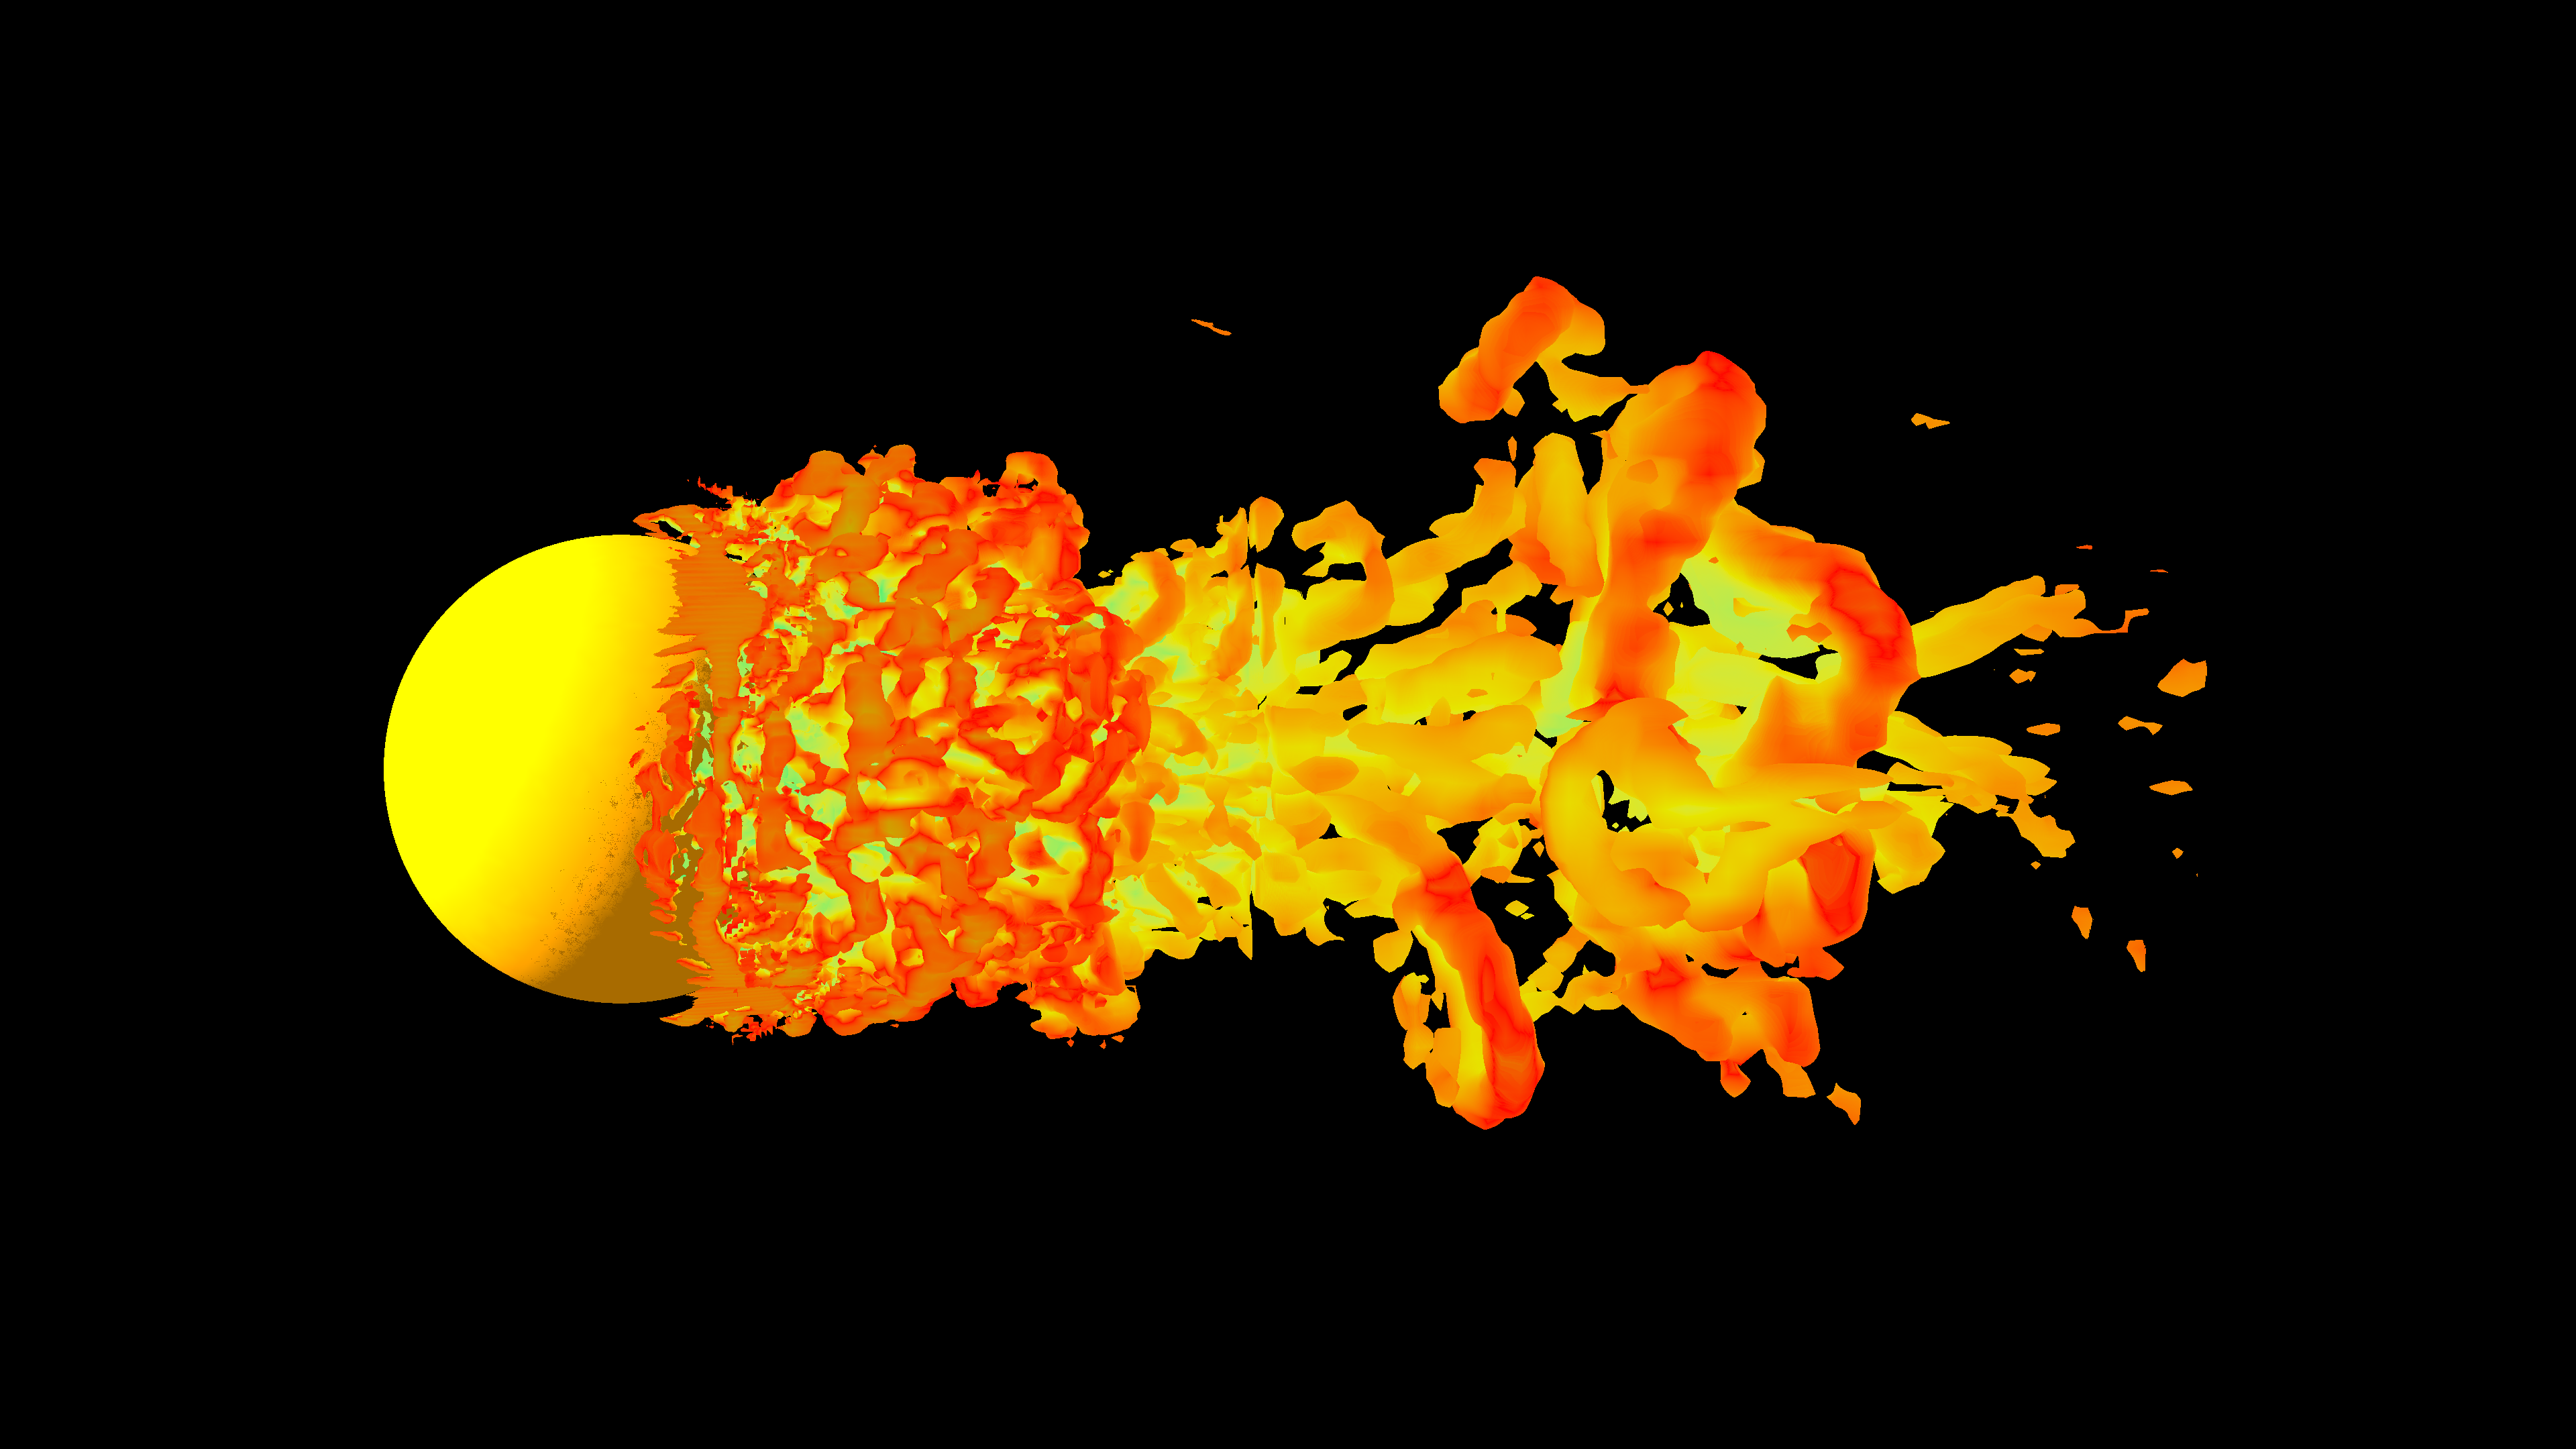
\includegraphics[width=0.45\textwidth]{./image/mutli_small_4k_8_filter_0.006}
        \caption{Multi-resolution small field, 4k resolution, $ \frac{dx}{8} $ step size with object filtering (iso-value = 0.006)}\label{fig:figure5}
    \end{figure}

    \begin{figure}[H]
        \centering
        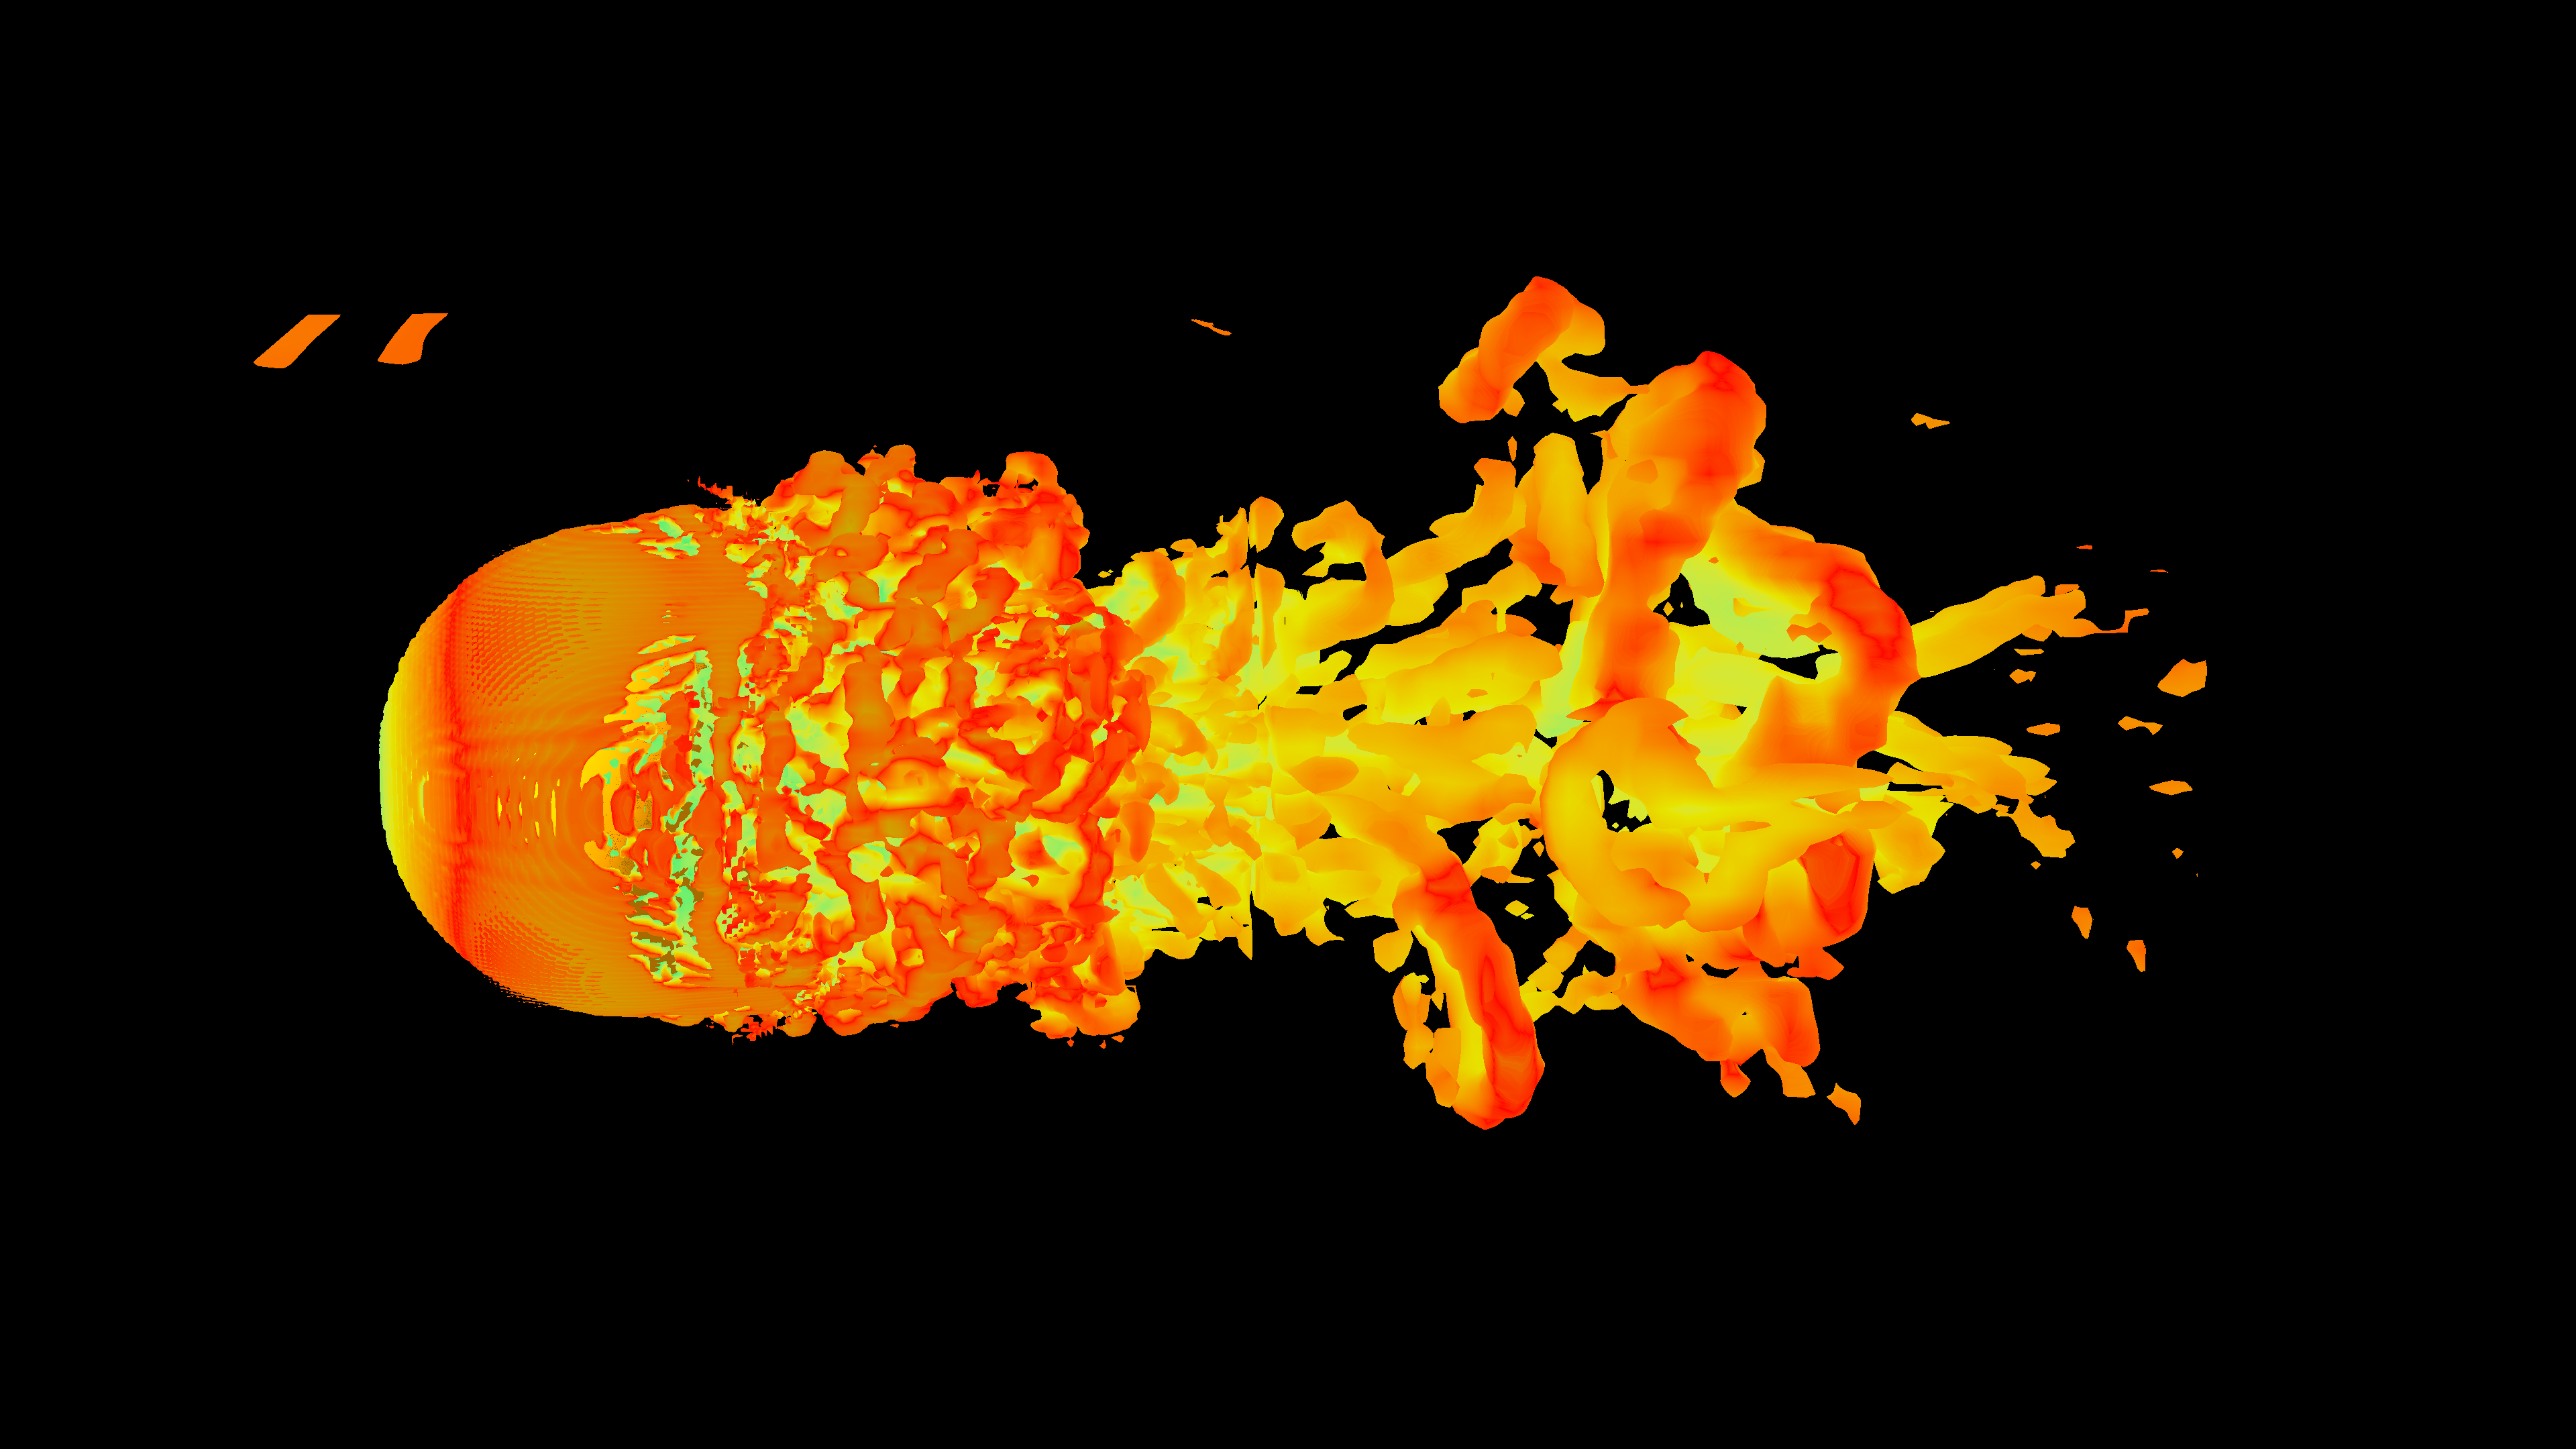
\includegraphics[width=0.45\textwidth]{./image/multi_small_4k_8_no_filter_0.006}
        \caption{Multi-resolution small field, 4k resolution, $ \frac{dx}{8} $ step size without object filtering (iso-value = 0.006)}\label{fig:figure6}
    \end{figure}

    \begin{figure}[H]
        \centering
        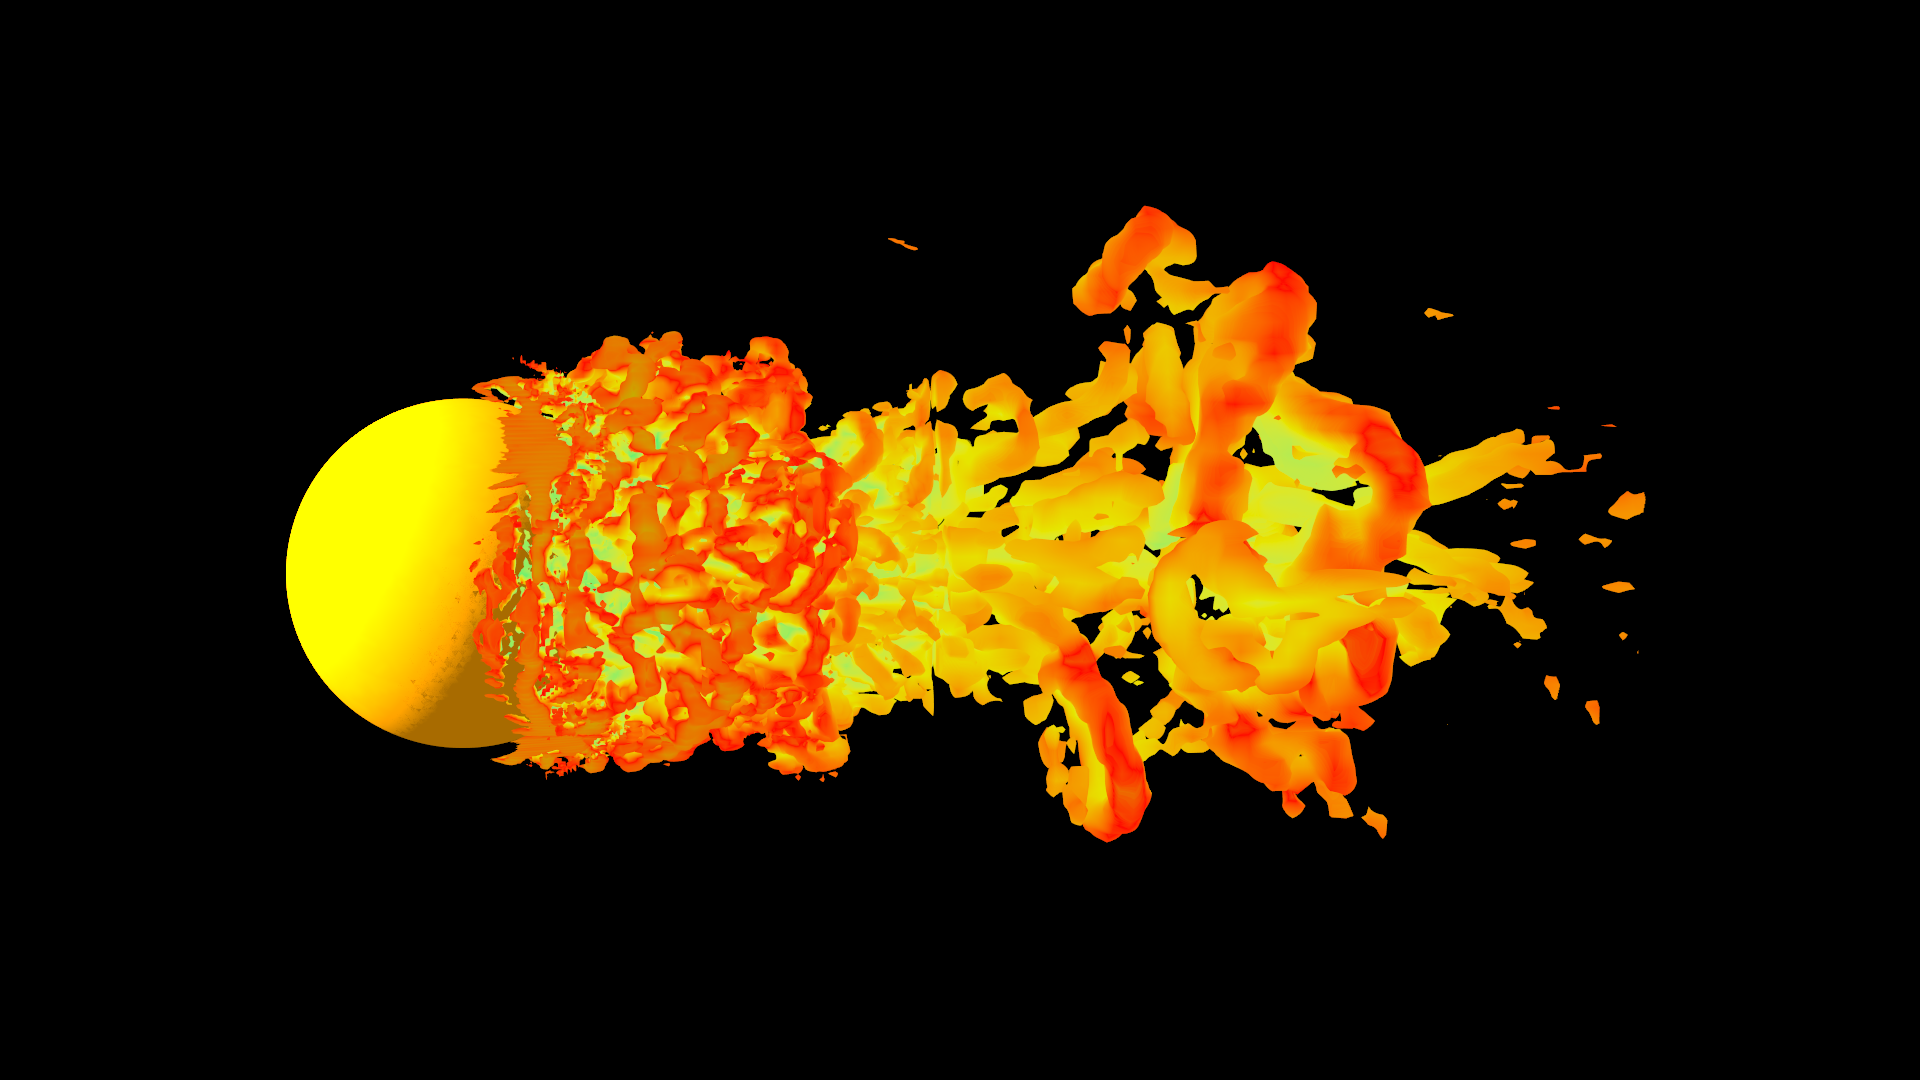
\includegraphics[width=0.45\textwidth]{./image/multi_small_1080p_8_filter_0.006_4XRES}
        \caption{Multi-resolution small field, 1080p resolution, $ \frac{dx}{8} $ step size with object filtering and 4X super resolution anti-aliasing (iso-value = 0.006)}\label{fig:figure7}
    \end{figure}

    \begin{figure}[H]
        \centering
        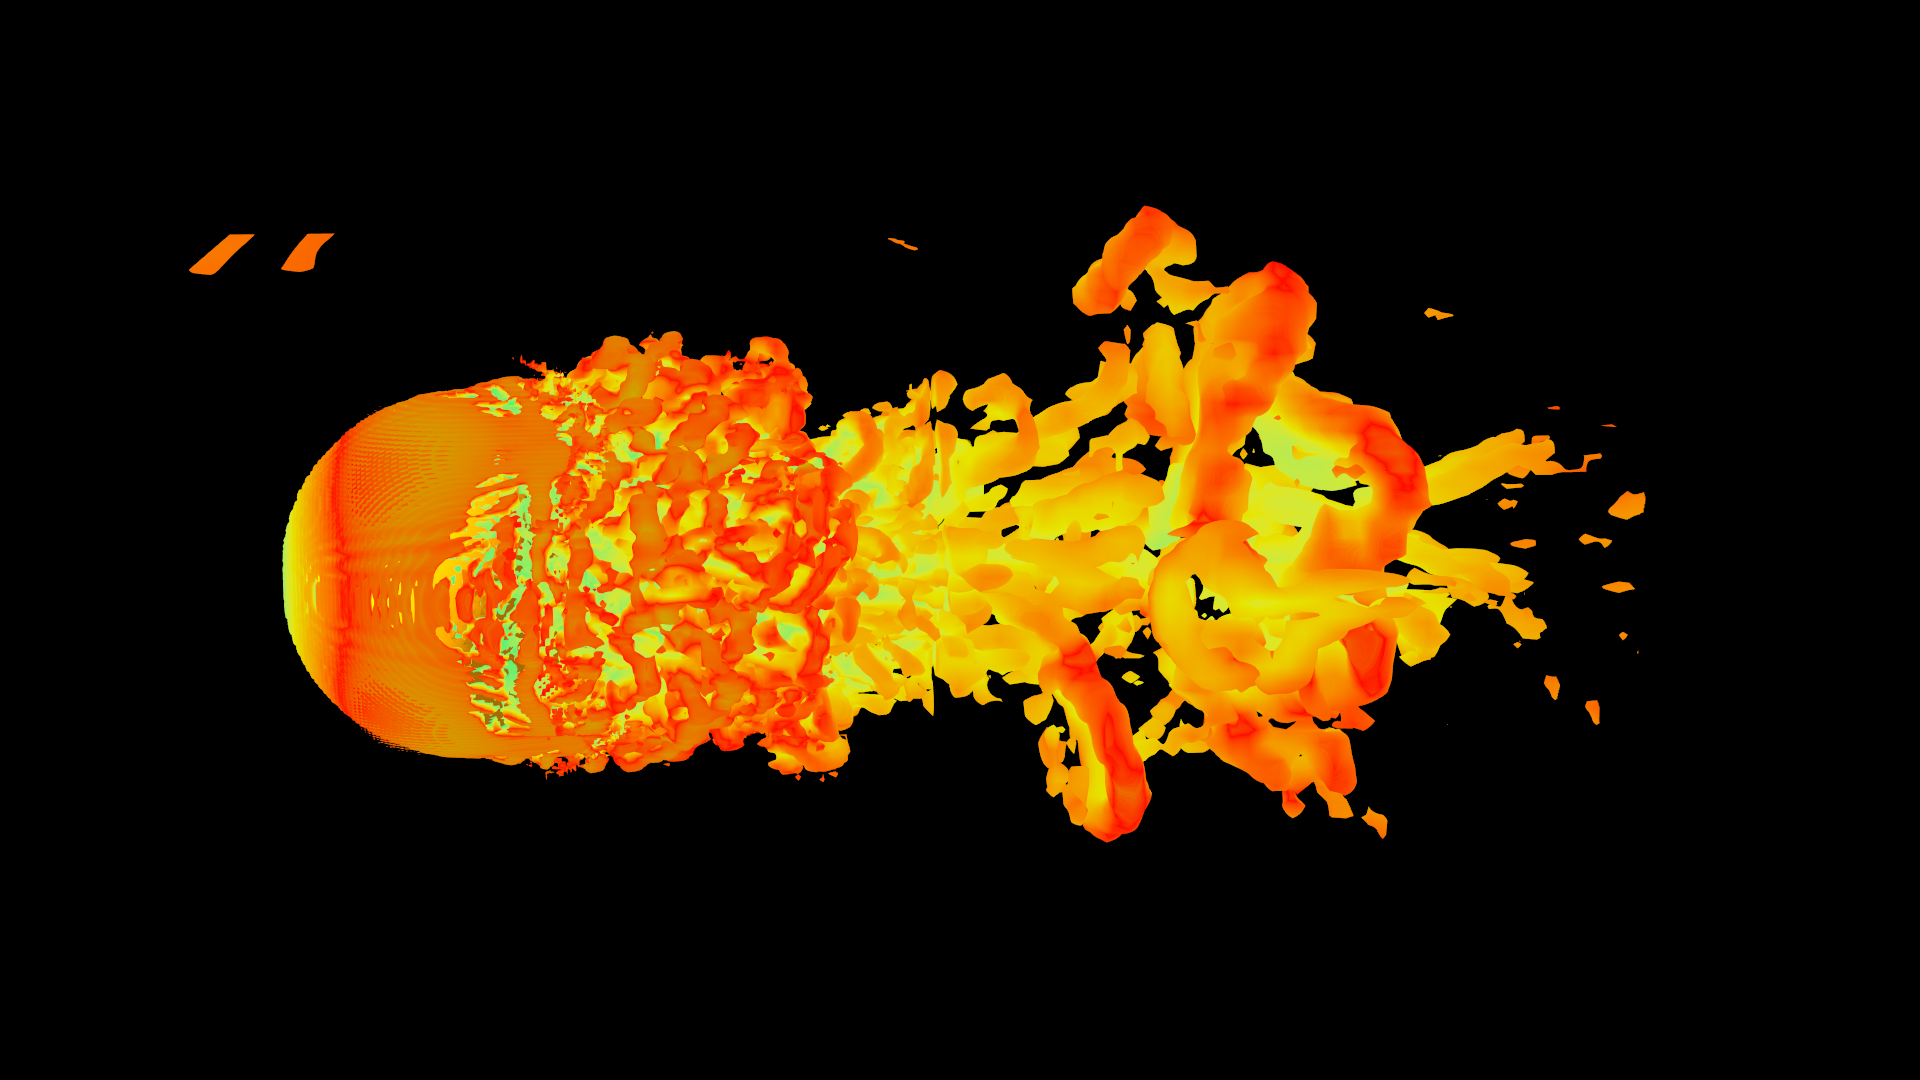
\includegraphics[width=0.45\textwidth]{./image/multi_small_1080p_8_no_filter_0.006_4XRES}
        \caption{Multi-resolution small field, 1080p resolution, $ \frac{dx}{8} $ step size without object filtering and 4X super resolution anti-aliasing (iso-value = 0.006)}\label{fig:figure8}
    \end{figure}

    \subsection{single-resolution big model}\label{subsec:single-resolution-big-model}
    \begin{figure}[H]
        \centering
        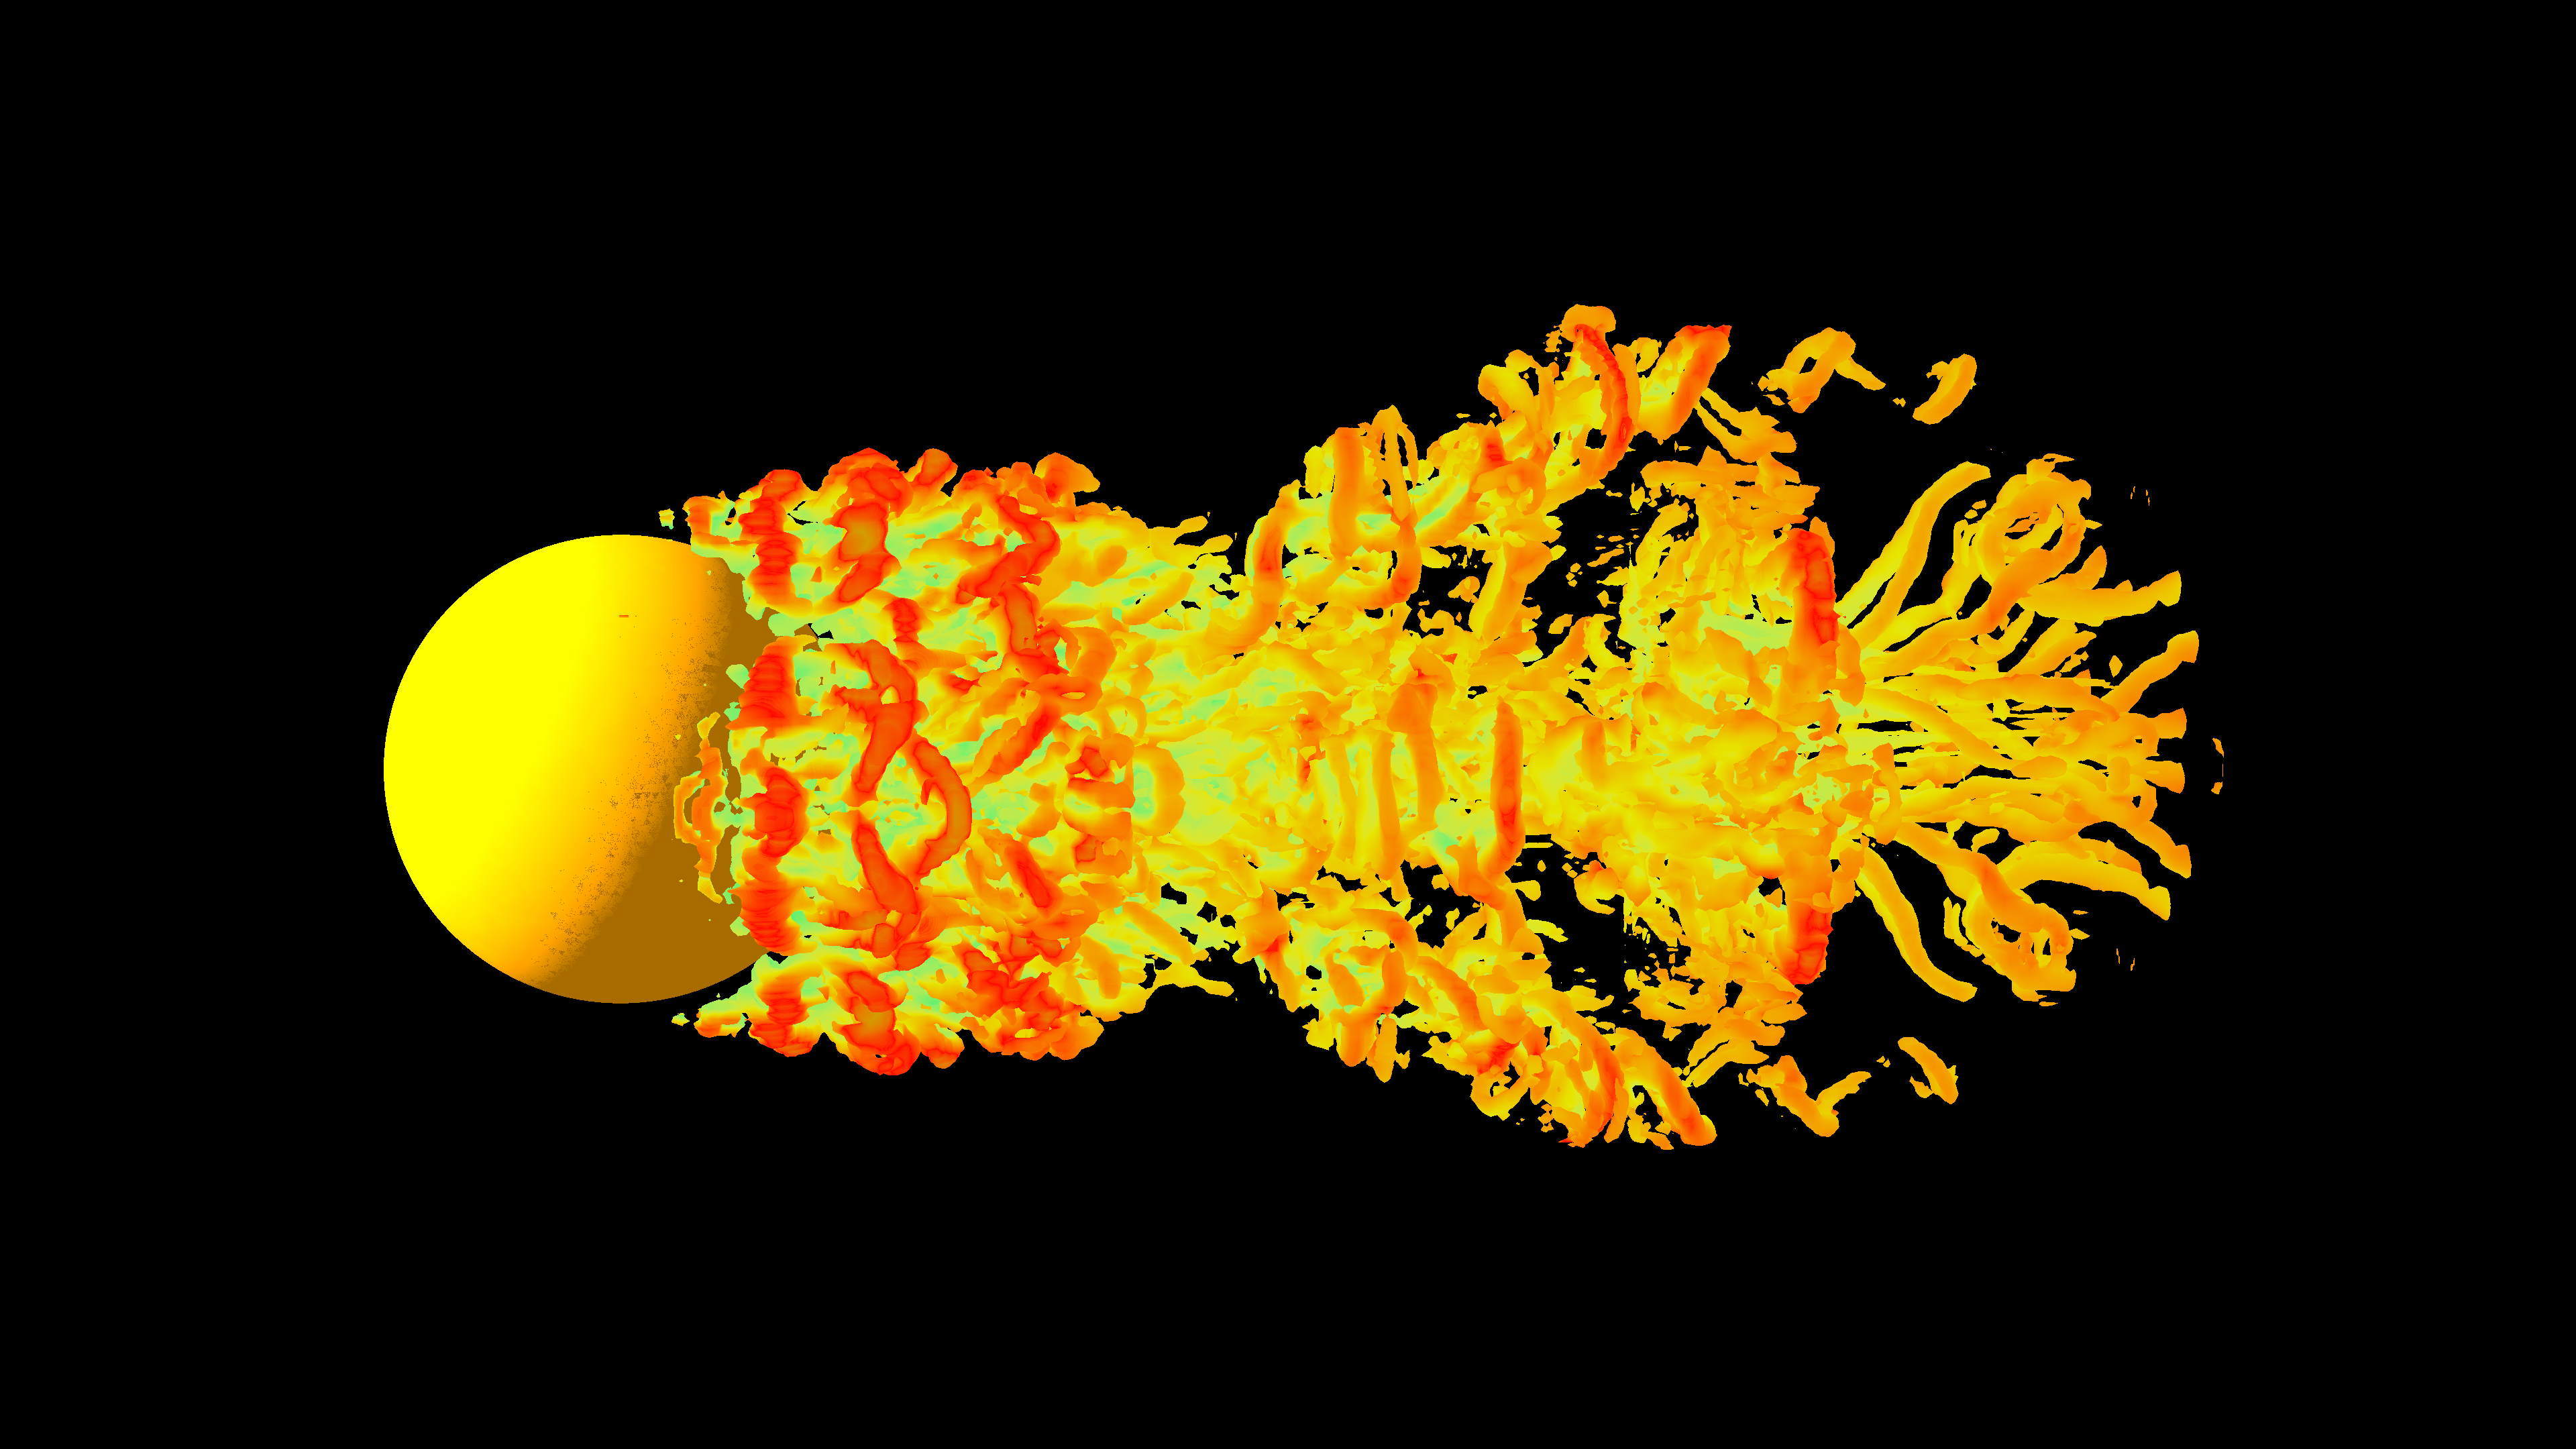
\includegraphics[width=0.45\textwidth]{./image/single_big_4k_8_filter_0.04}
        \caption{Single-resolution big field, 4k resolution, $ \frac{dx}{8} $ step size with object filtering (iso-value = 0.04)}\label{fig:figure9}
    \end{figure}

    \begin{figure}[H]
        \centering
        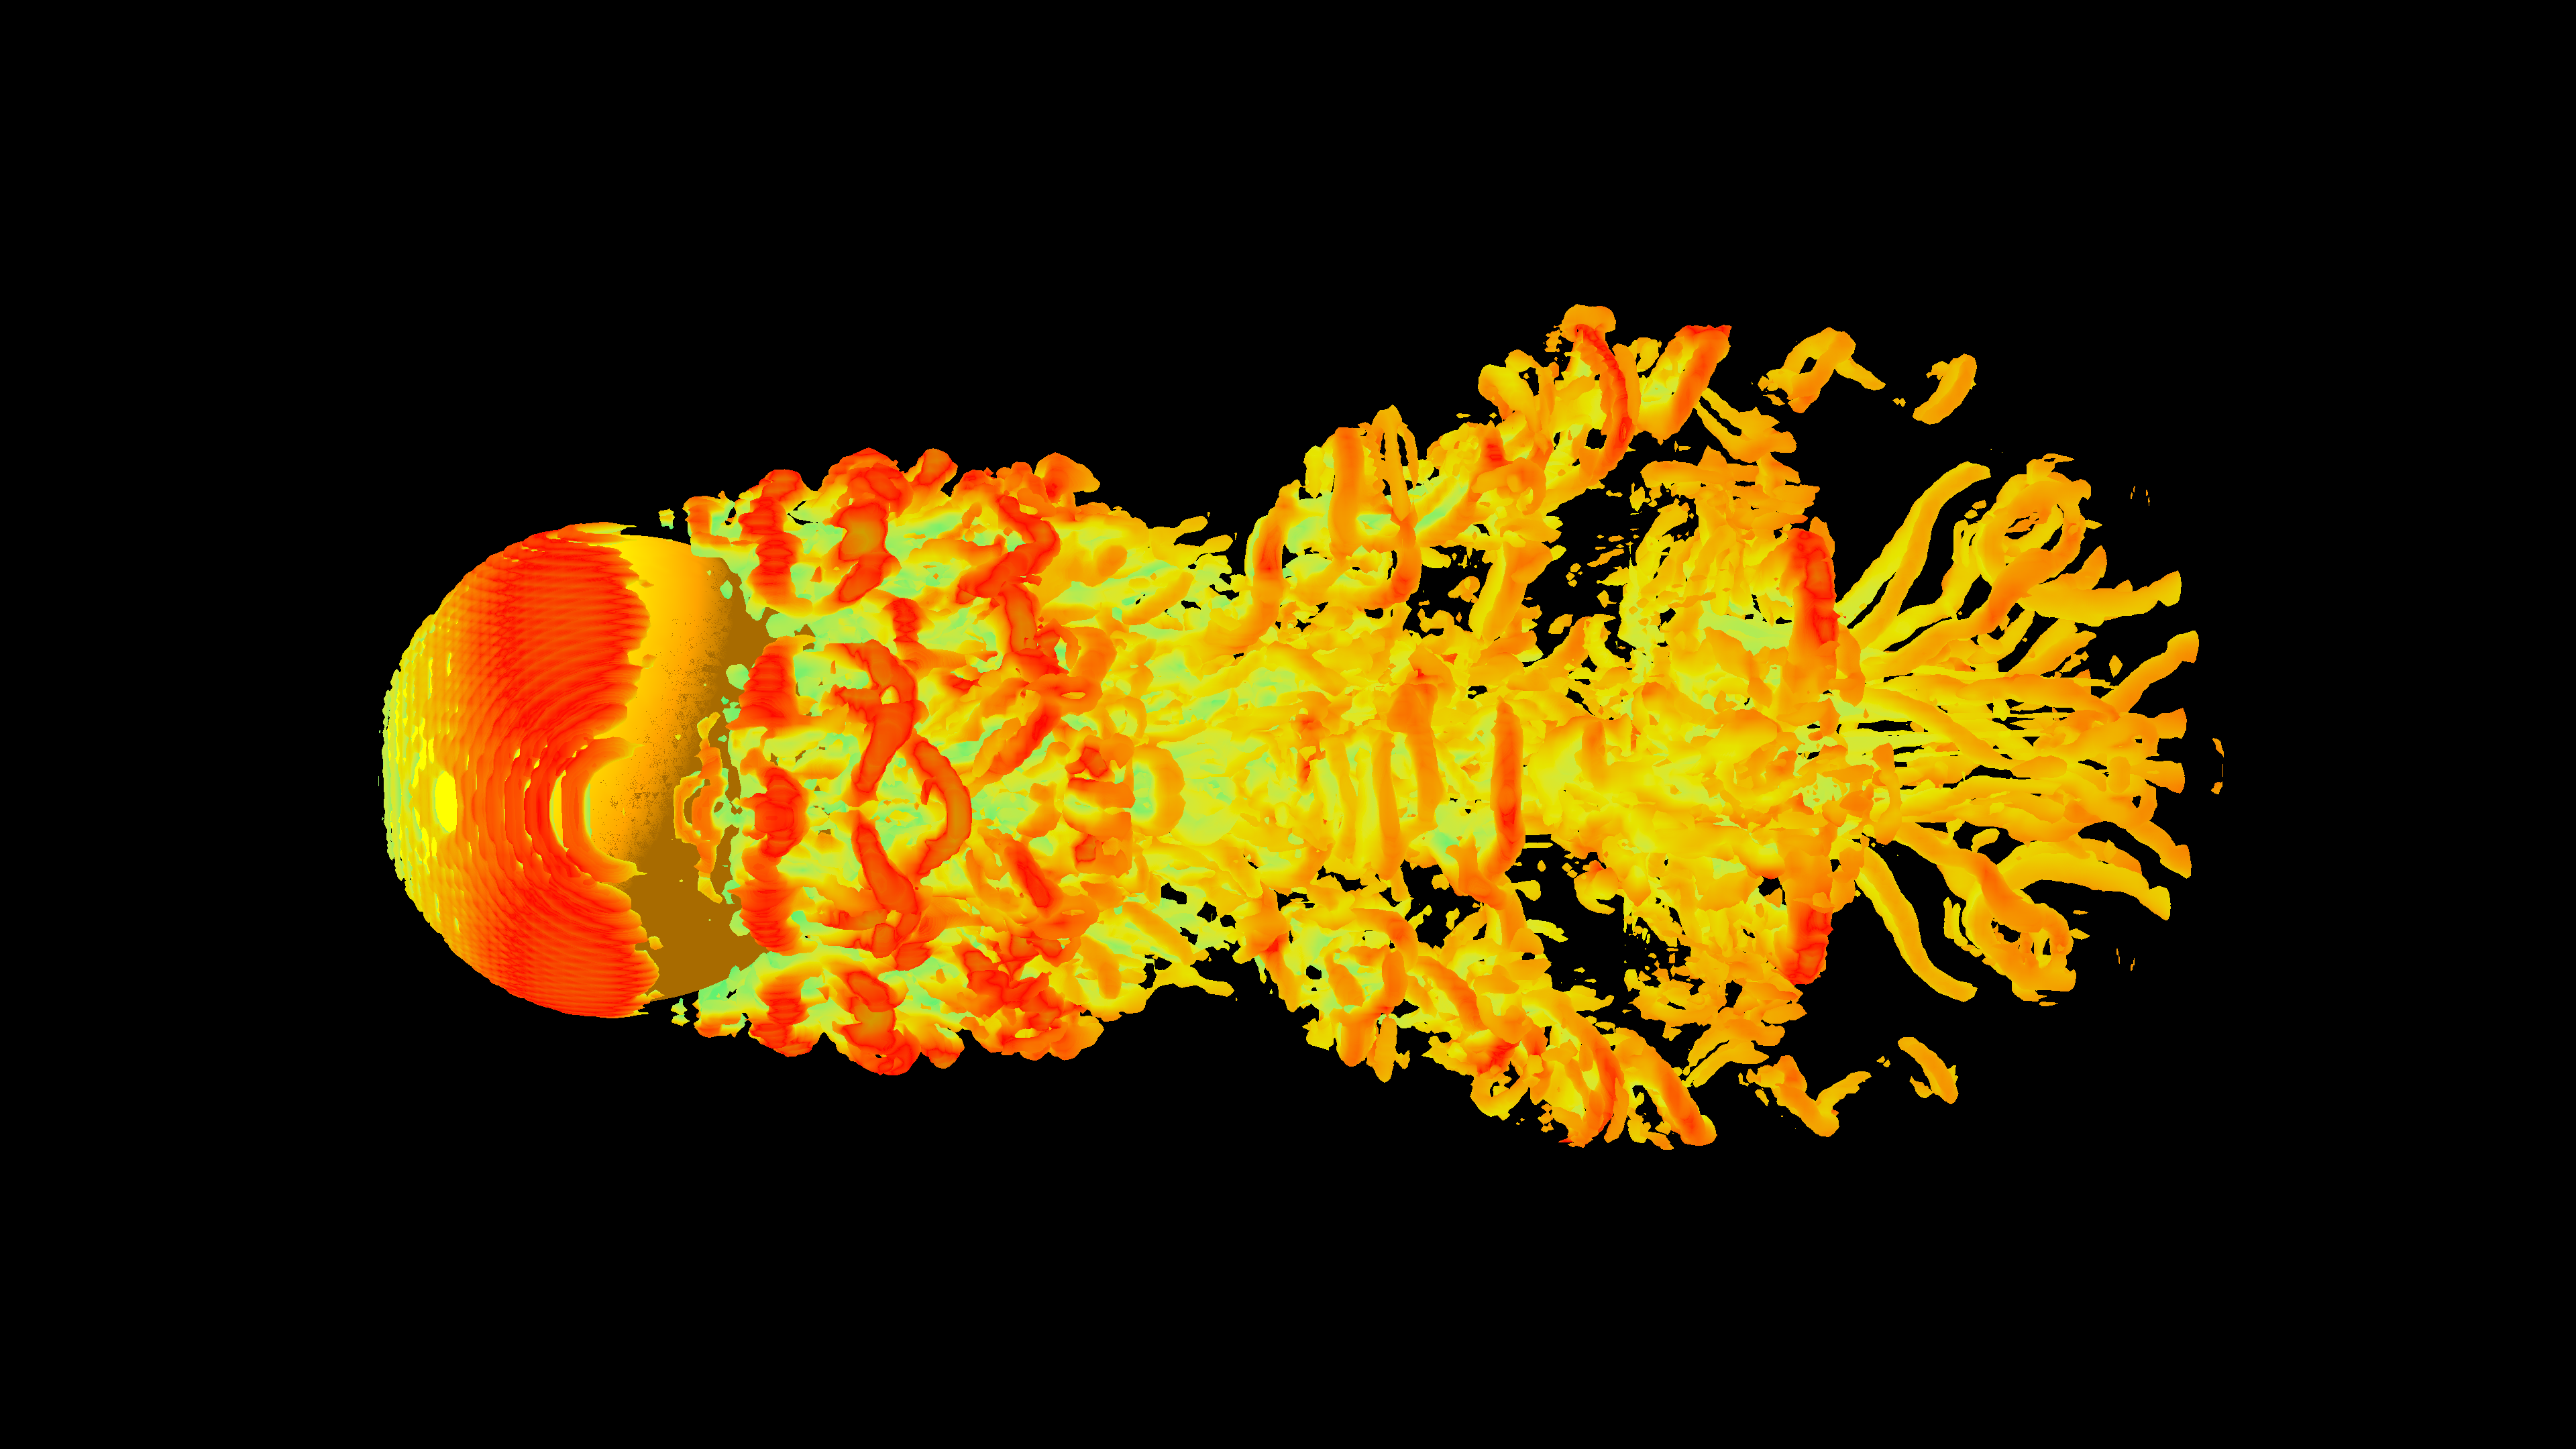
\includegraphics[width=0.45\textwidth]{./image/single_big_4k_8_no_filter_0.04}
        \caption{Single-resolution big field, 4k resolution, $ \frac{dx}{8} $ step size without object filtering (iso-value = 0.04)}\label{fig:figure10}
    \end{figure}

    \begin{figure}[H]
        \centering
        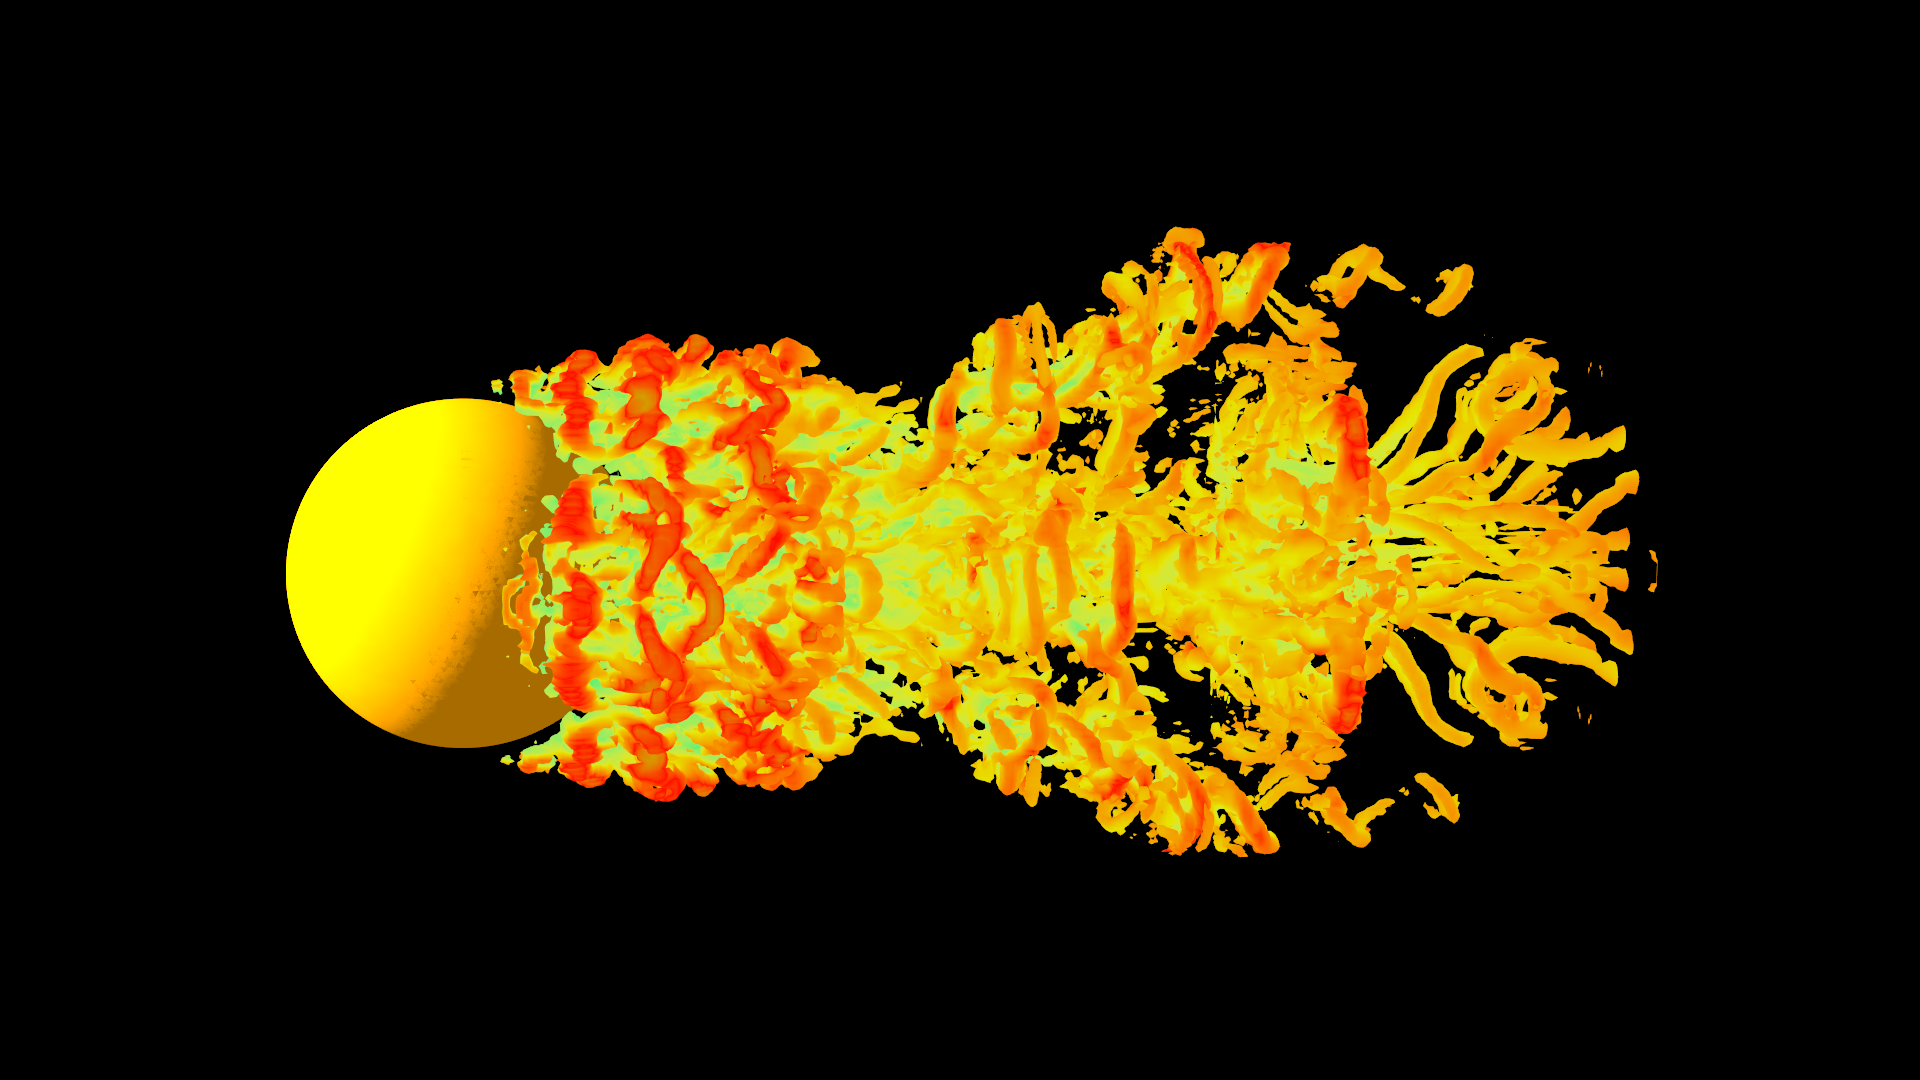
\includegraphics[width=0.45\textwidth]{./image/single_big_1080p_8_filter_0.04_4XRES}
        \caption{Single-resolution big field, 1080p resolution, $ \frac{dx}{8} $ step size with object filtering and 4X super resolution anti-aliasing (iso-value = 0.04)}\label{fig:figure11}
    \end{figure}

    \begin{figure}[H]
        \centering
        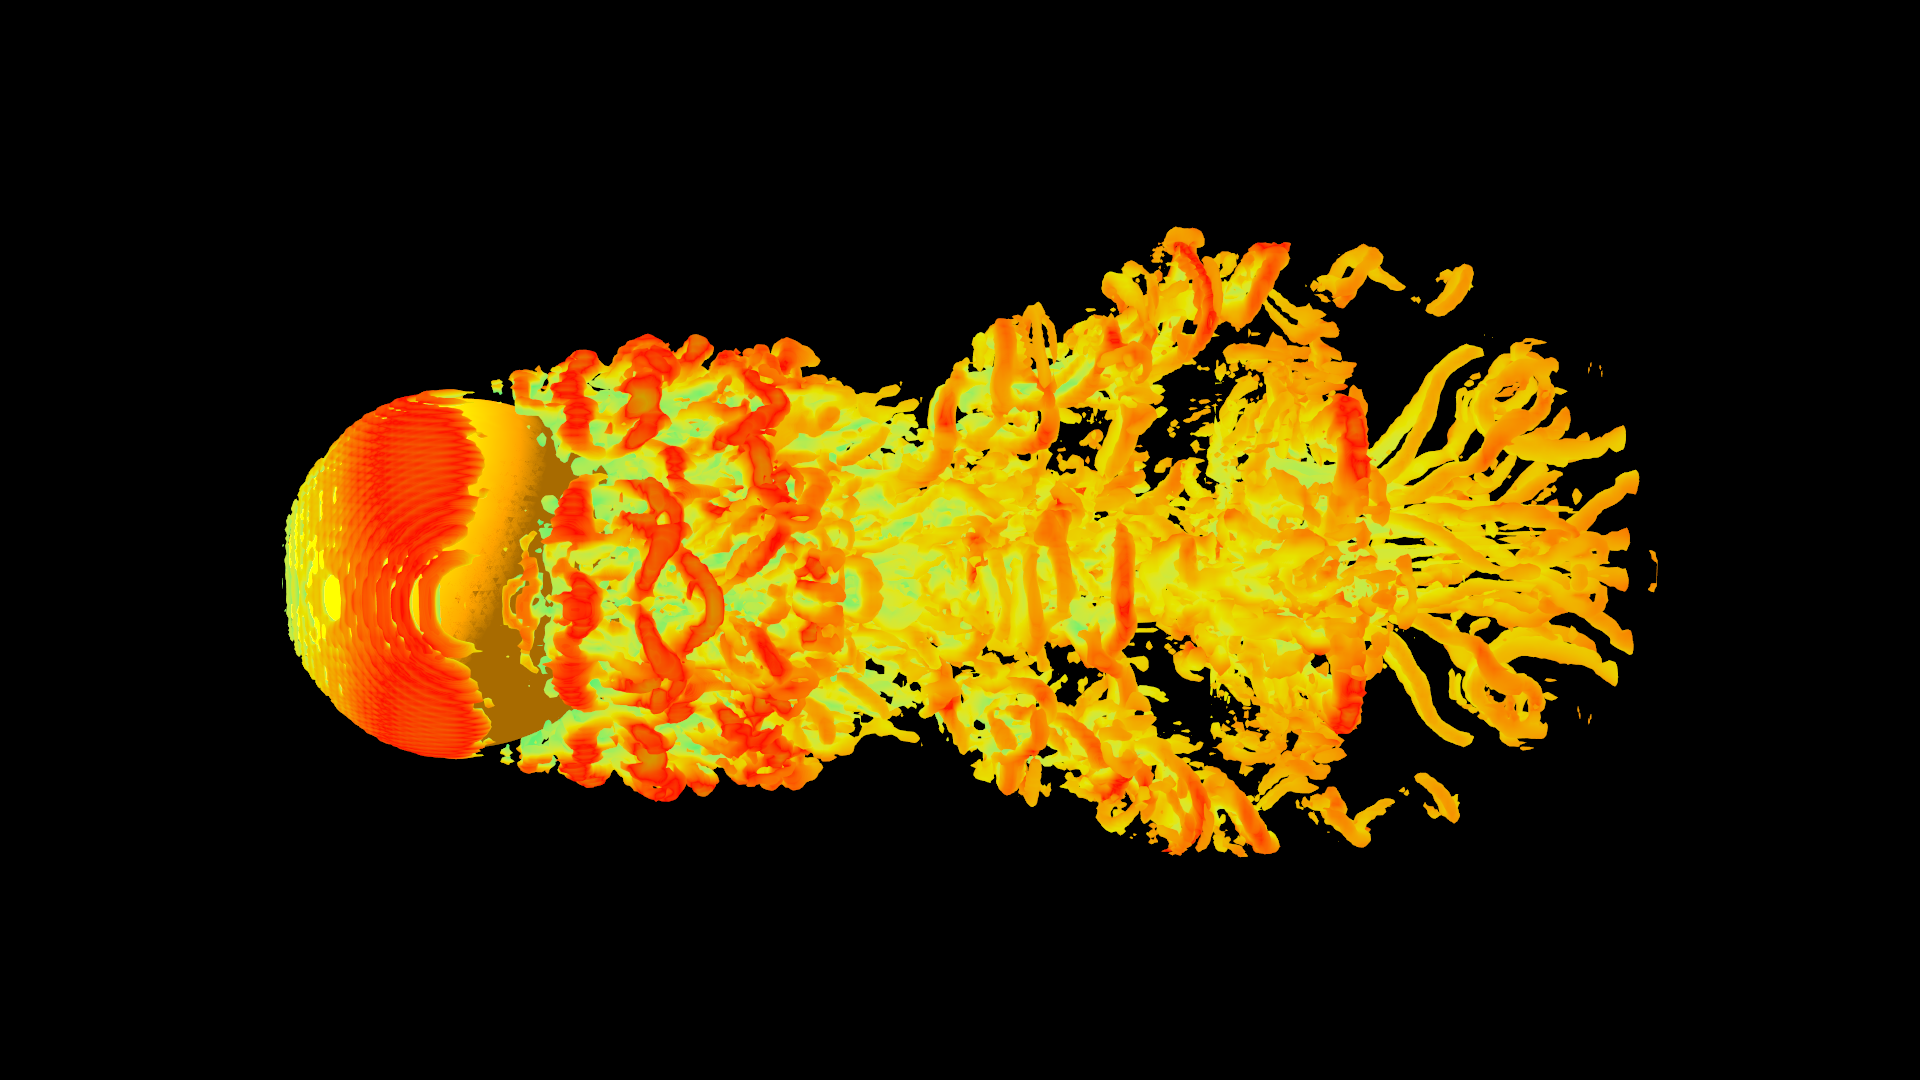
\includegraphics[width=0.45\textwidth]{./image/single_big_1080p_8_no_filter_0.04_4XRES}
        \caption{Single-resolution big field, 1080p resolution, $ \frac{dx}{8} $ step size without object filtering and 4X super resolution anti-aliasing (iso-value = 0.04)}\label{fig:figure12}
    \end{figure}

    \subsection{single-resolution small model}\label{subsec:single-resolution-small-model}
    \begin{figure}[H]
        \centering
        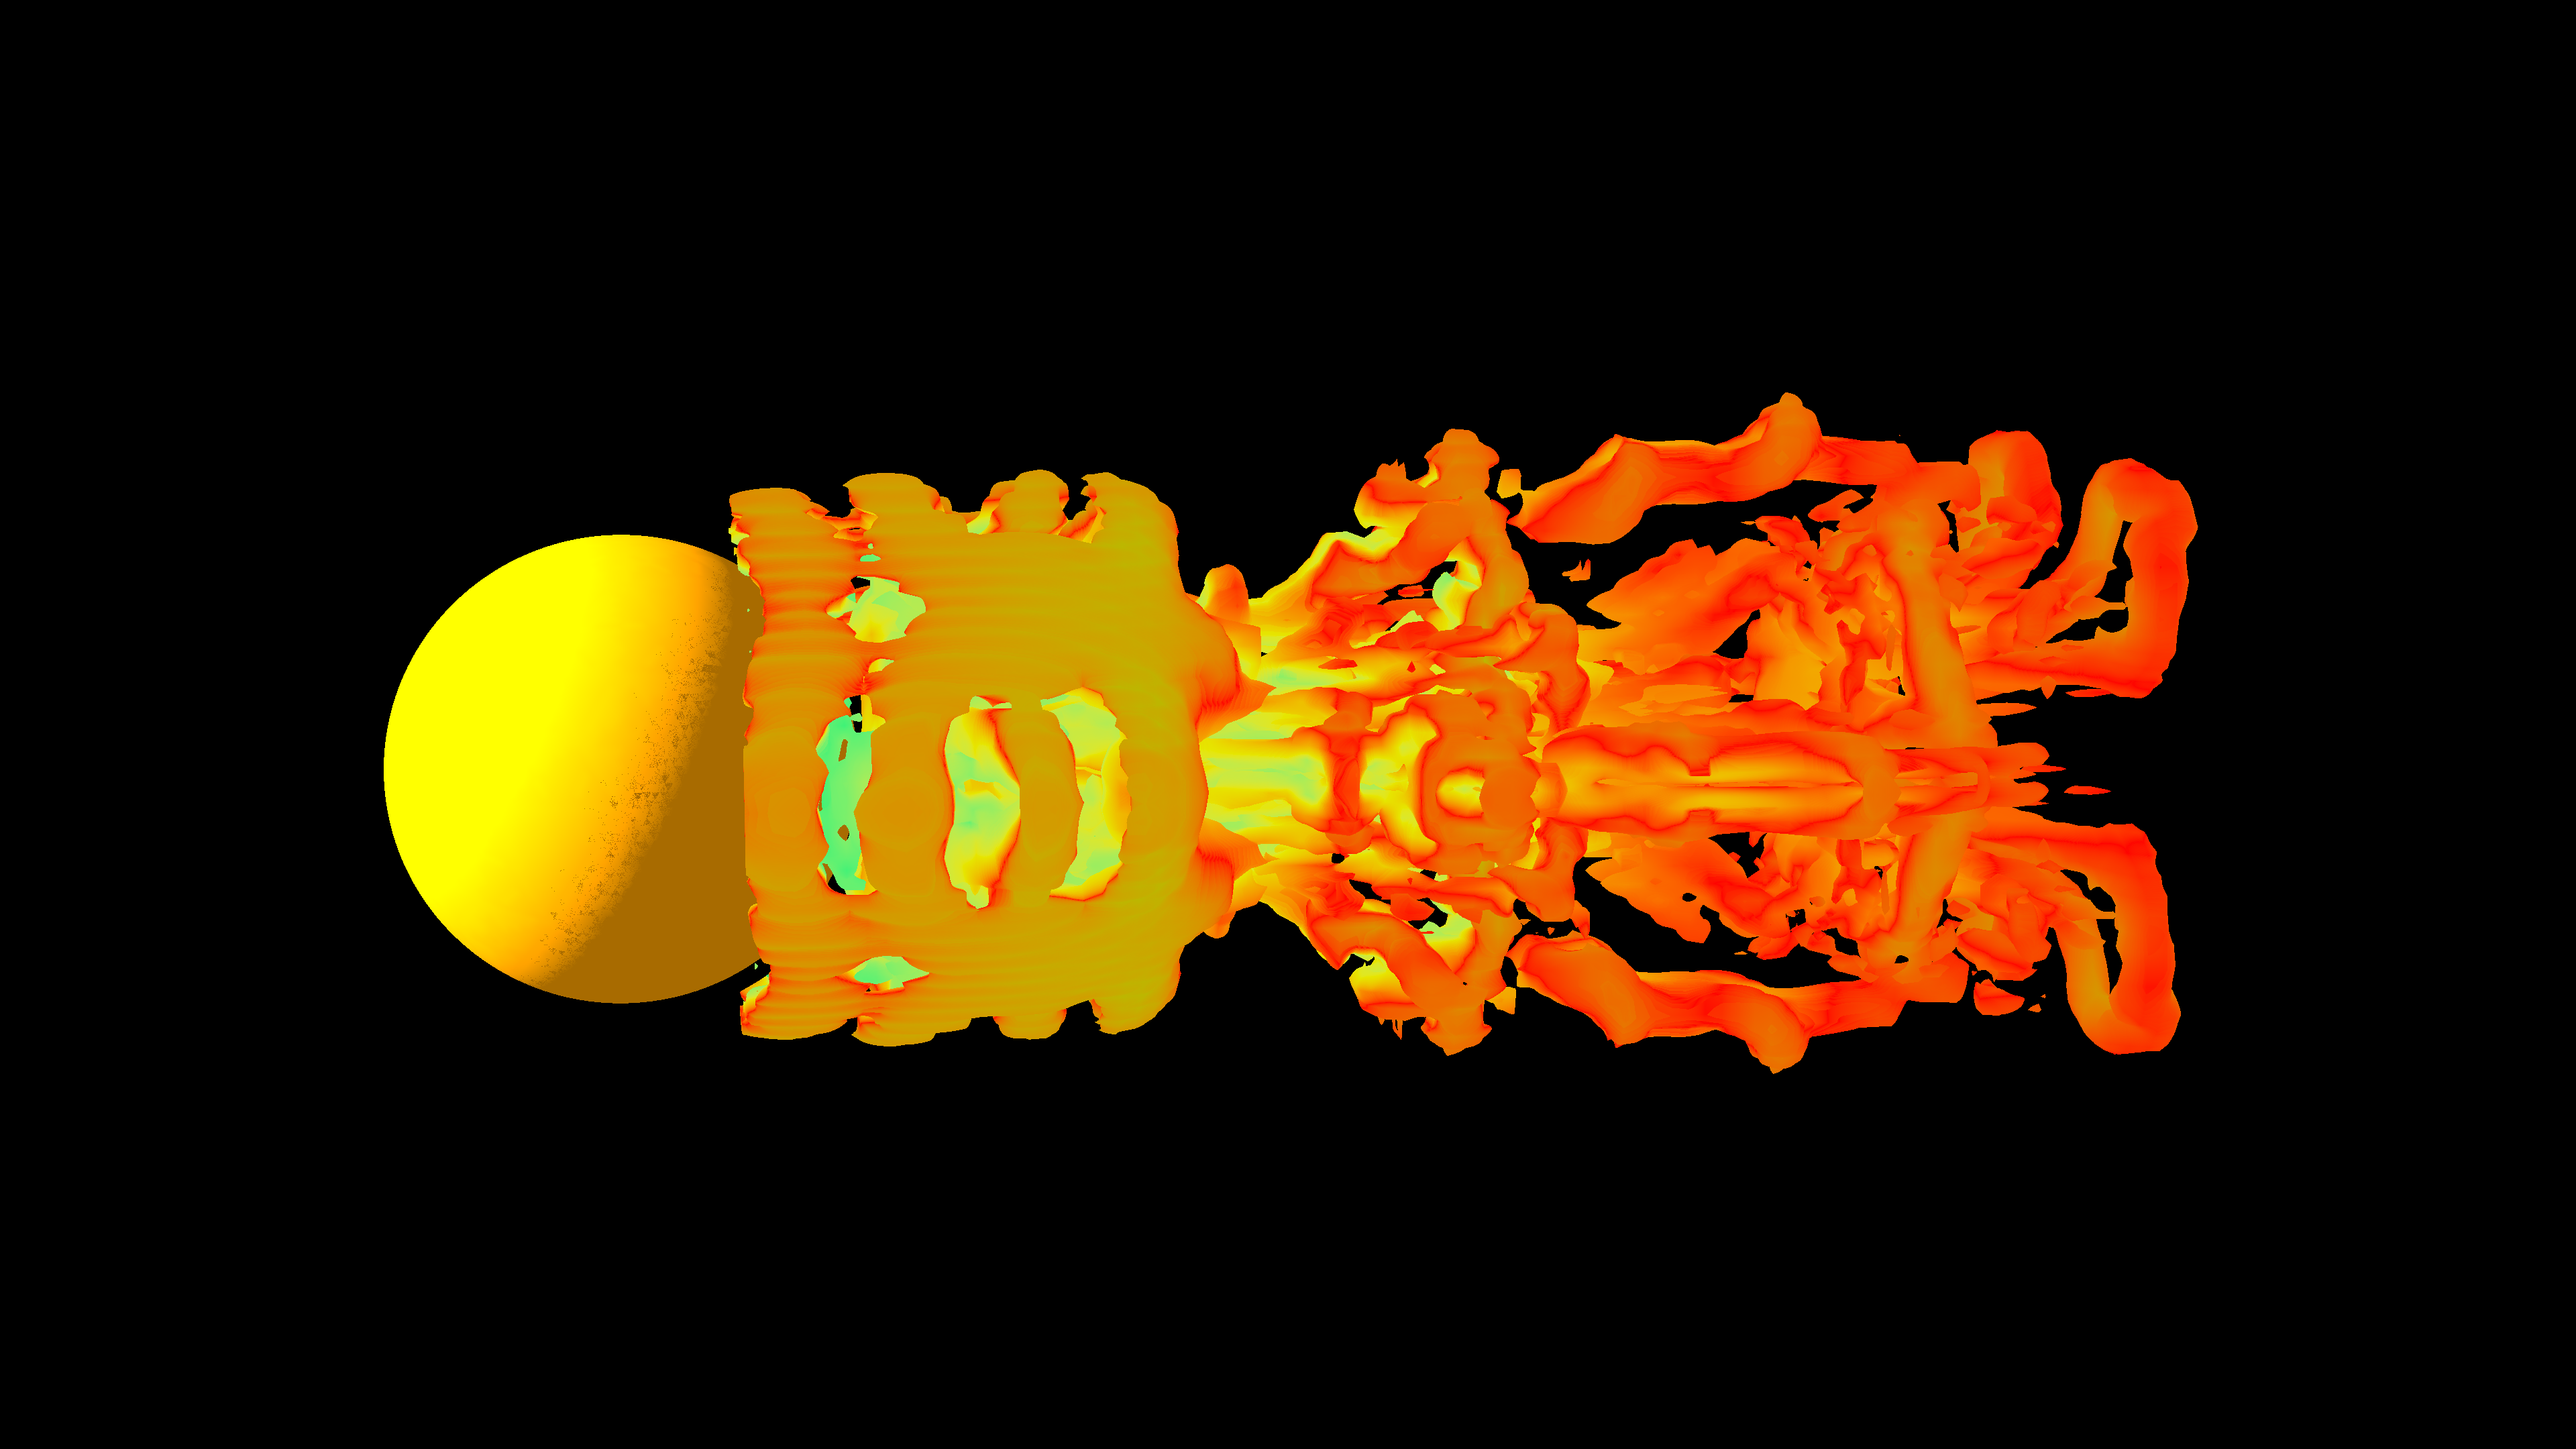
\includegraphics[width=0.45\textwidth]{./image/single_small_4k_8_filter_0.002}
        \caption{Single-resolution small field, 4k resolution, $ \frac{dx}{8} $ step size with object filtering (iso-value = 0.002)}\label{fig:figure13}
    \end{figure}

    \begin{figure}[H]
        \centering
        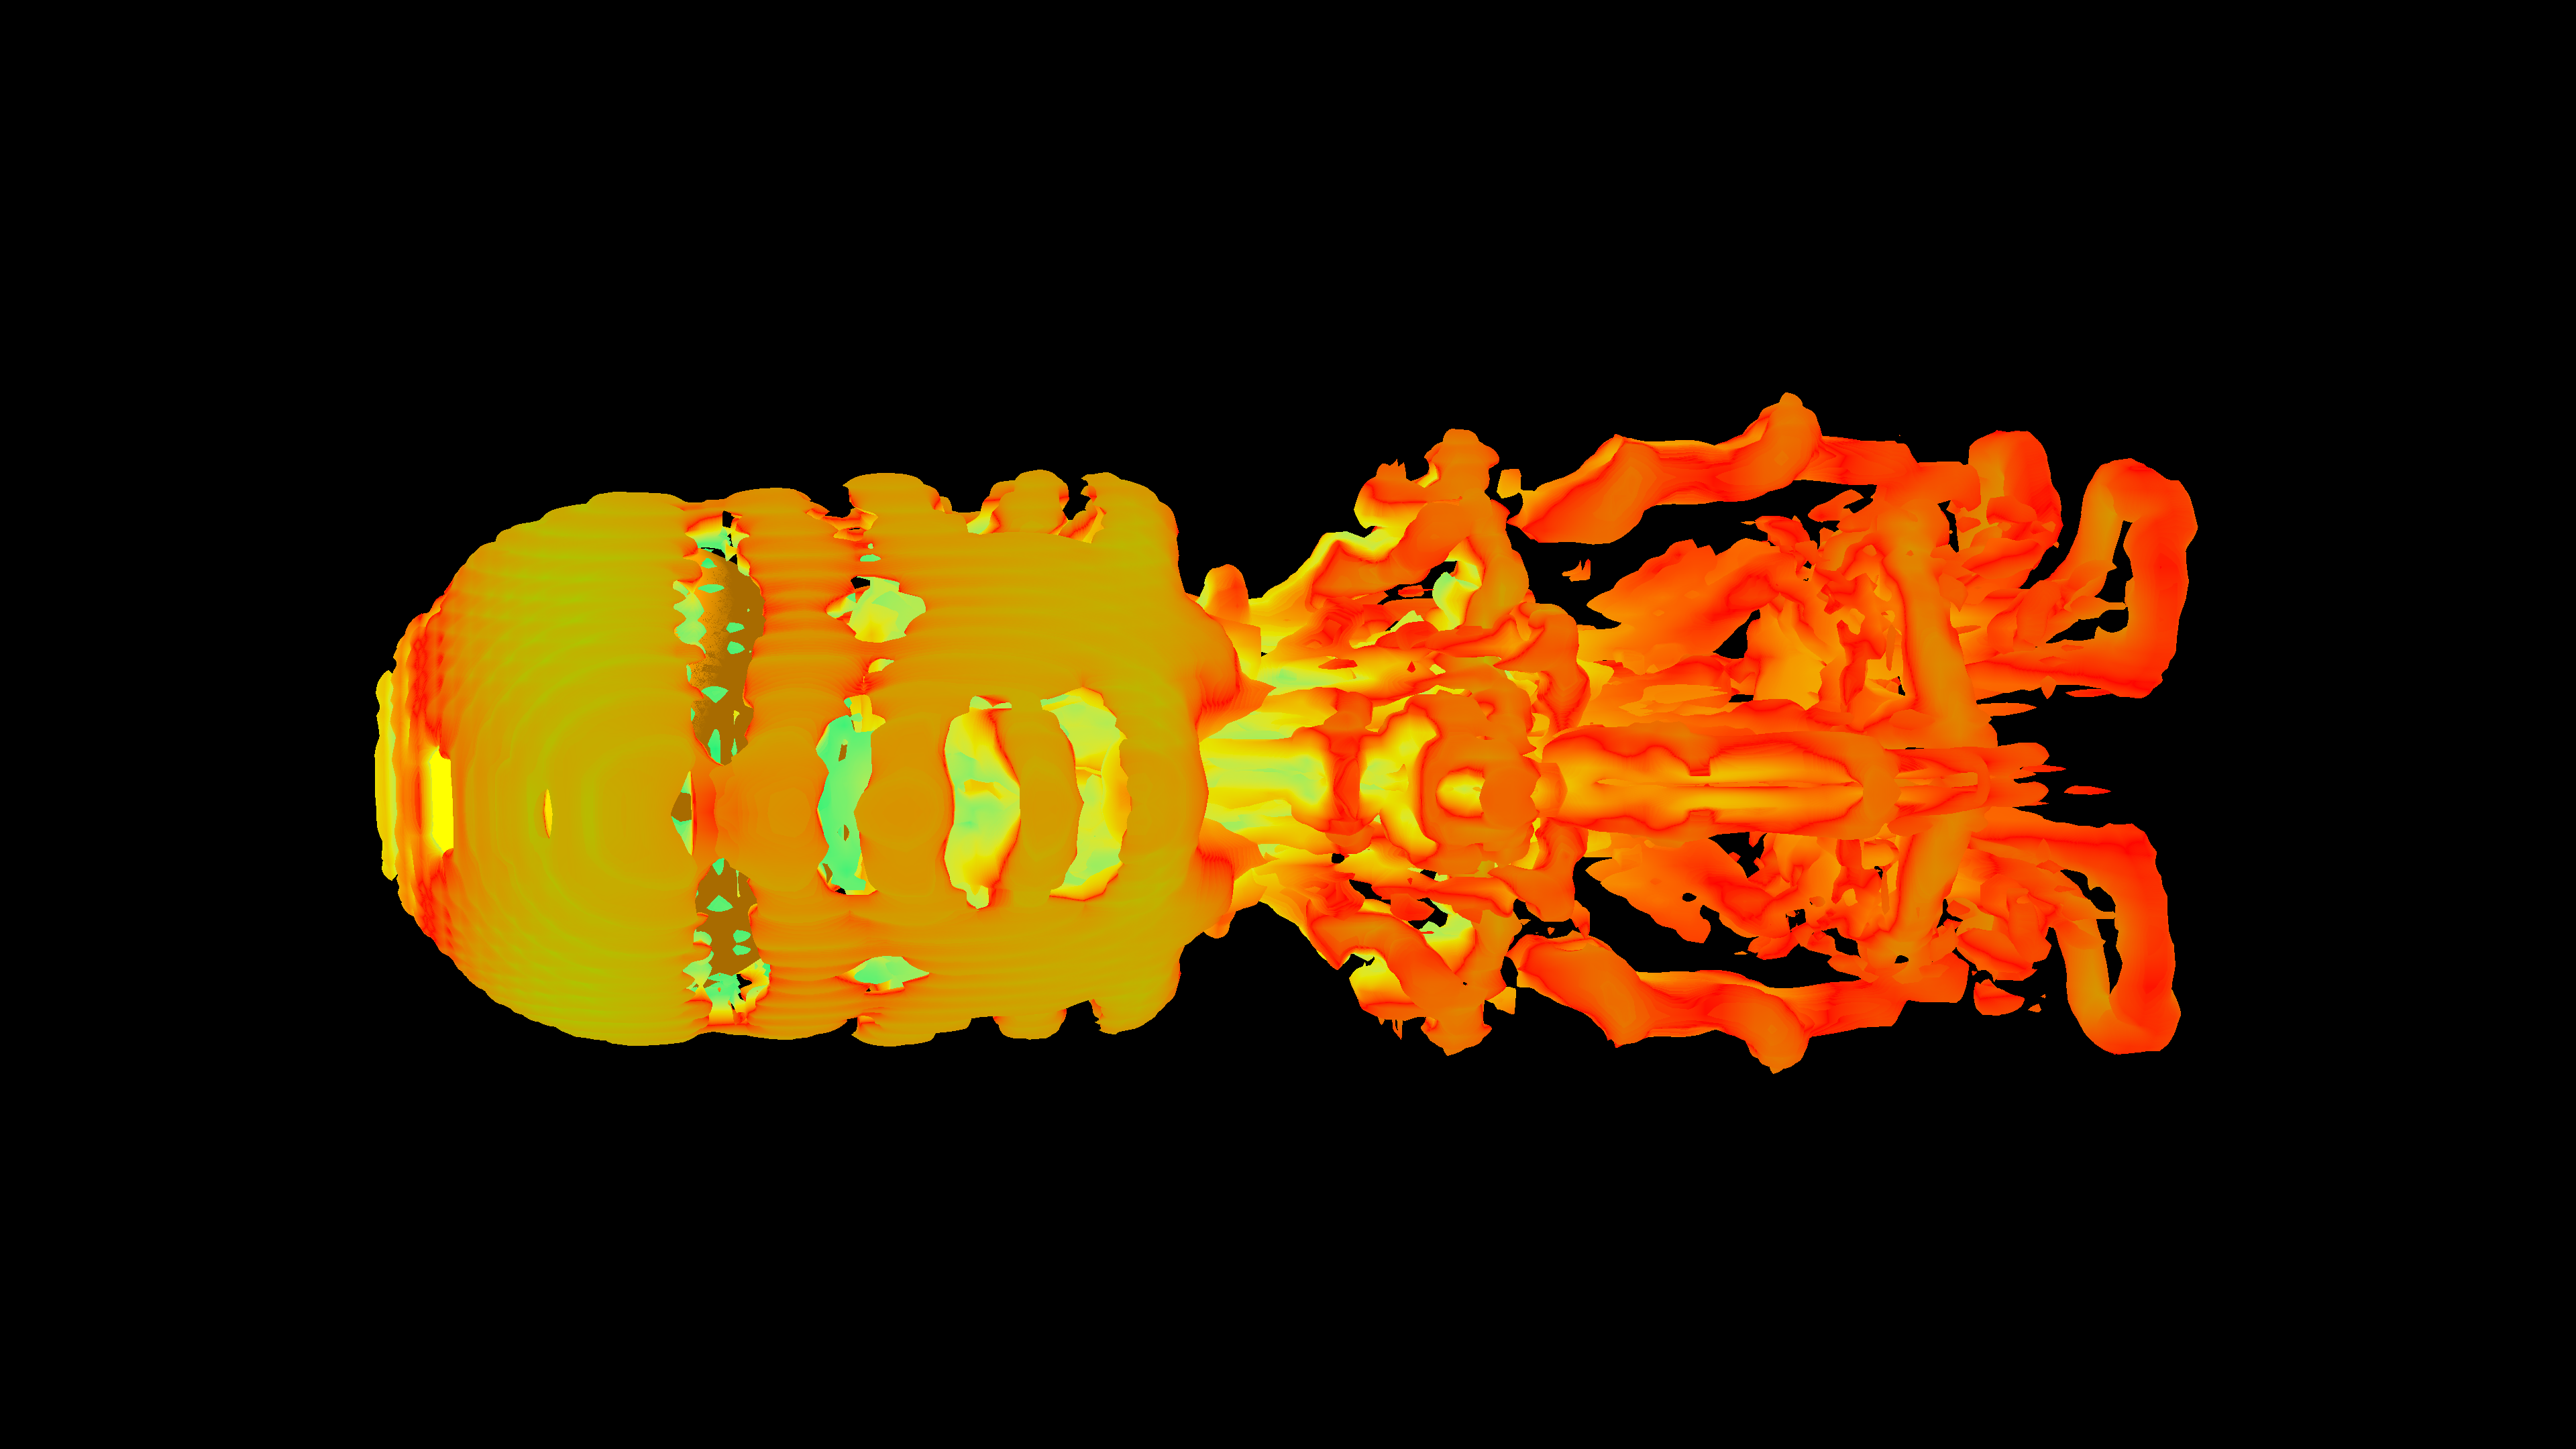
\includegraphics[width=0.45\textwidth]{./image/single_small_4k_8_no_filter_0.002}
        \caption{Single-resolution small field, 4k resolution, $ \frac{dx}{8} $ step size without object filtering (iso-value = 0.002)}\label{fig:figure14}
    \end{figure}

    \begin{figure}[H]
        \centering
        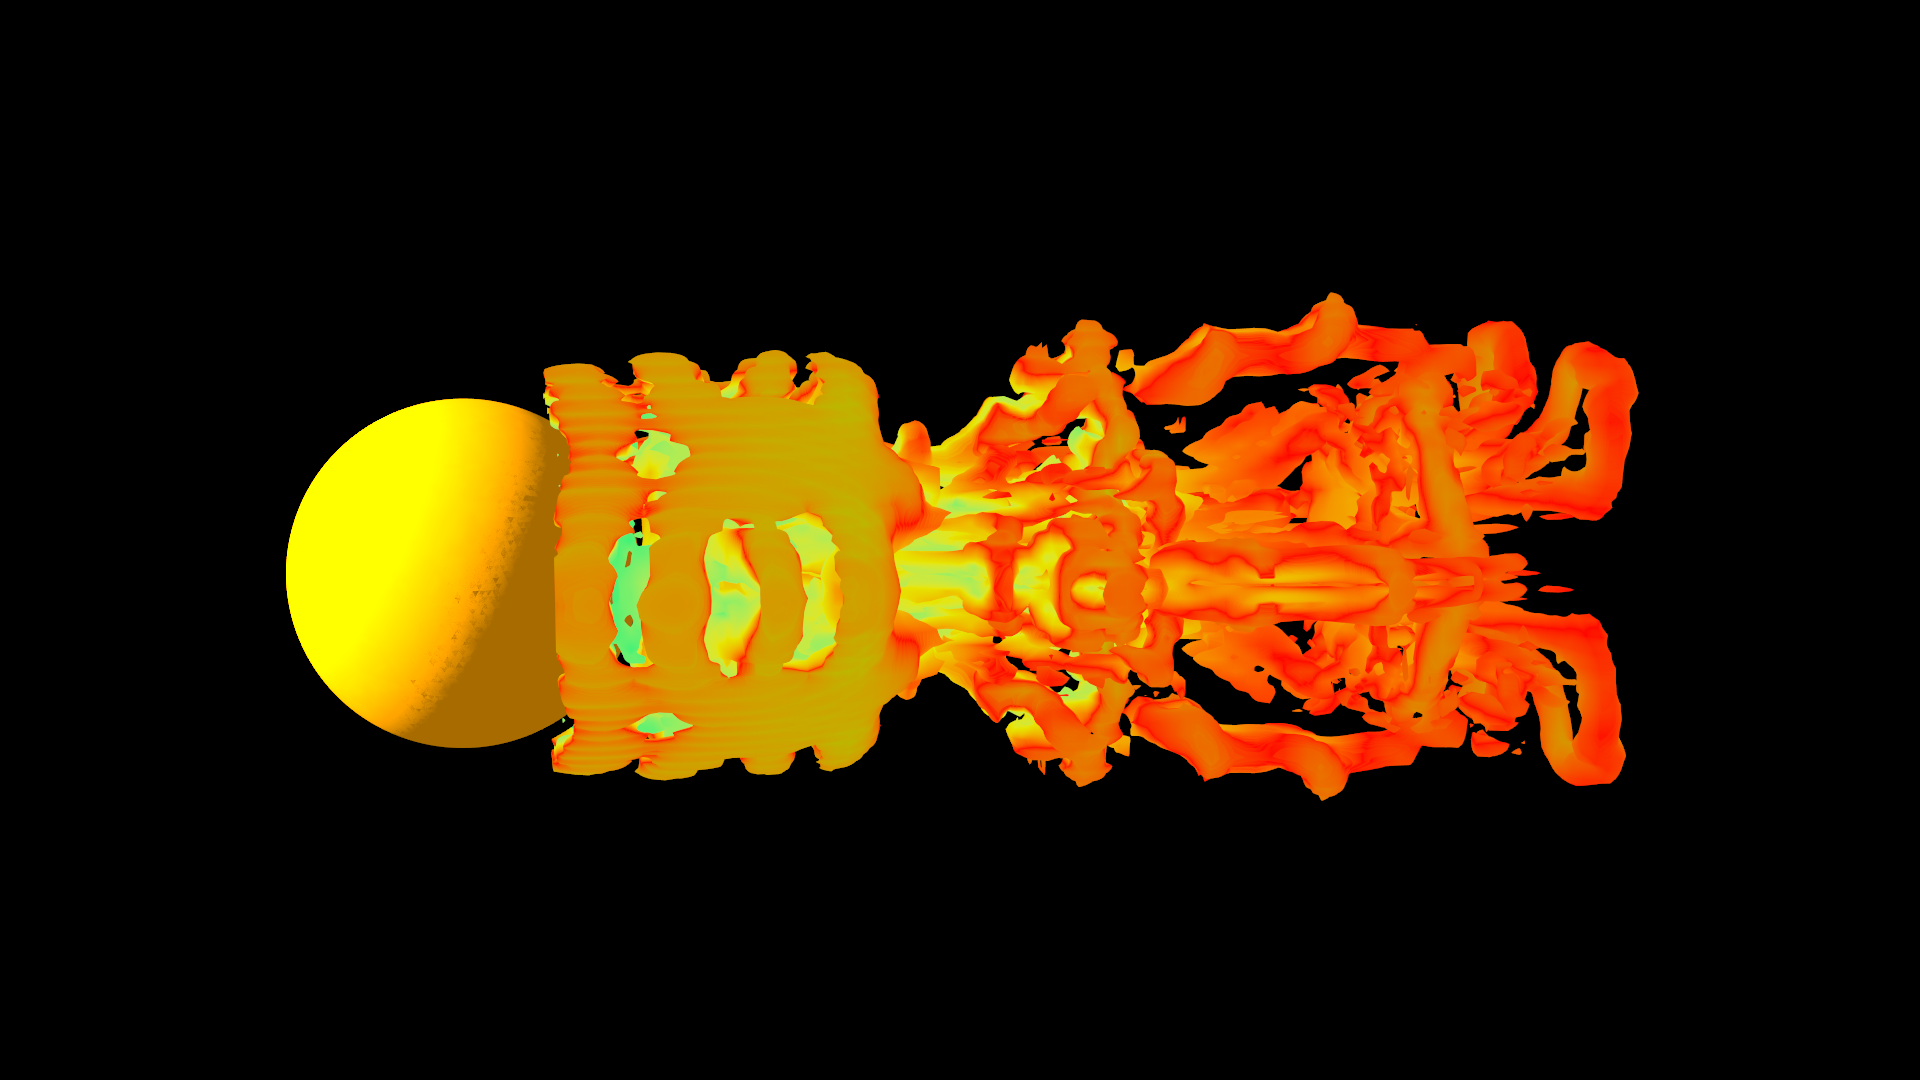
\includegraphics[width=0.45\textwidth]{./image/single_small_1080p_8_filter_0.002_4XRES}
        \caption{Single-resolution small field, 1080p resolution, $ \frac{dx}{8} $ step size with object filtering and 4X super resolution anti-aliasing (iso-value = 0.002)}\label{fig:figure15}
    \end{figure}

    \begin{figure}[H]
        \centering
        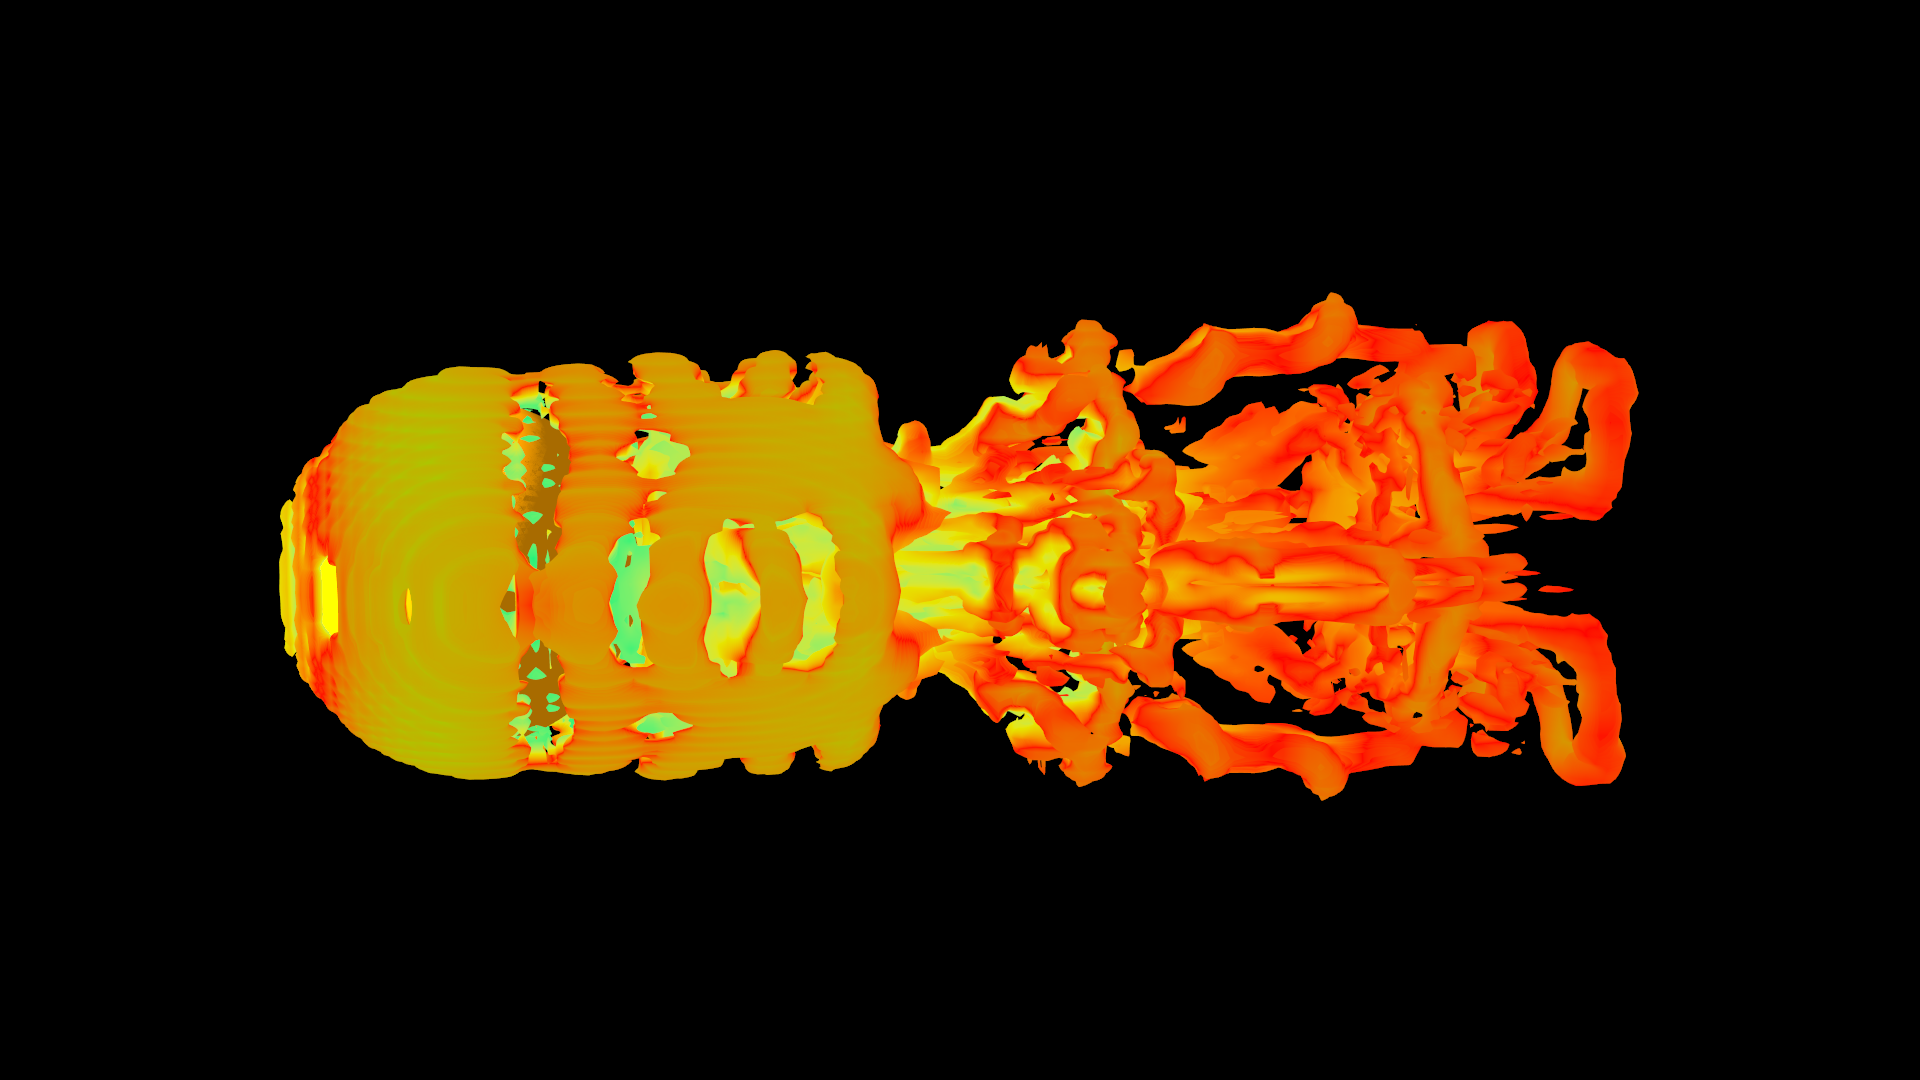
\includegraphics[width=0.45\textwidth]{./image/single_small_1080p_8_no_filter_0.002_4XRES}
        \caption{Single-resolution small field, 1080p resolution, $ \frac{dx}{8} $ step size without object filtering and 4X super resolution anti-aliasing (iso-value = 0.002)}\label{fig:figure16}
    \end{figure}


    \section{Division of work}\label{sec:division-of-work}

    \subsection{Bingnan Li's part}\label{subsec:bingnan-li's-part}
    \begin{itemize}
        \item volume rendering framework construction
        \item q-criteria calculation and gradient calculation
        \item object filtering
        \item object rendering
    \end{itemize}

    \subsection{Suting Chen's part}\label{subsec:suting-chen's-part}
    \begin{itemize}
        \item k-d tree construction
        \item Multi-resolution model framework construction
        \item opacity and color transfer function design
        \item provide rendering hardware
    \end{itemize}


\end{document}
